\documentclass[]{article}
\usepackage{lmodern}
\usepackage{amssymb,amsmath}
\usepackage{ifxetex,ifluatex}
\usepackage{fixltx2e} % provides \textsubscript
\ifnum 0\ifxetex 1\fi\ifluatex 1\fi=0 % if pdftex
  \usepackage[T1]{fontenc}
  \usepackage[utf8]{inputenc}
\else % if luatex or xelatex
  \ifxetex
    \usepackage{mathspec}
  \else
    \usepackage{fontspec}
  \fi
  \defaultfontfeatures{Ligatures=TeX,Scale=MatchLowercase}
\fi
% use upquote if available, for straight quotes in verbatim environments
\IfFileExists{upquote.sty}{\usepackage{upquote}}{}
% use microtype if available
\IfFileExists{microtype.sty}{%
\usepackage[]{microtype}
\UseMicrotypeSet[protrusion]{basicmath} % disable protrusion for tt fonts
}{}
\PassOptionsToPackage{hyphens}{url} % url is loaded by hyperref
\usepackage[unicode=true]{hyperref}
\hypersetup{
            pdftitle={Analyzing Data from the MIDFIELD Project},
            pdfauthor={Javier Alvarez, Leah Hunt, and Joshua Kwak},
            pdfborder={0 0 0},
            breaklinks=true}
\urlstyle{same}  % don't use monospace font for urls
\usepackage[margin=1in]{geometry}
\usepackage{color}
\usepackage{fancyvrb}
\newcommand{\VerbBar}{|}
\newcommand{\VERB}{\Verb[commandchars=\\\{\}]}
\DefineVerbatimEnvironment{Highlighting}{Verbatim}{commandchars=\\\{\}}
% Add ',fontsize=\small' for more characters per line
\usepackage{framed}
\definecolor{shadecolor}{RGB}{248,248,248}
\newenvironment{Shaded}{\begin{snugshade}}{\end{snugshade}}
\newcommand{\KeywordTok}[1]{\textcolor[rgb]{0.13,0.29,0.53}{\textbf{#1}}}
\newcommand{\DataTypeTok}[1]{\textcolor[rgb]{0.13,0.29,0.53}{#1}}
\newcommand{\DecValTok}[1]{\textcolor[rgb]{0.00,0.00,0.81}{#1}}
\newcommand{\BaseNTok}[1]{\textcolor[rgb]{0.00,0.00,0.81}{#1}}
\newcommand{\FloatTok}[1]{\textcolor[rgb]{0.00,0.00,0.81}{#1}}
\newcommand{\ConstantTok}[1]{\textcolor[rgb]{0.00,0.00,0.00}{#1}}
\newcommand{\CharTok}[1]{\textcolor[rgb]{0.31,0.60,0.02}{#1}}
\newcommand{\SpecialCharTok}[1]{\textcolor[rgb]{0.00,0.00,0.00}{#1}}
\newcommand{\StringTok}[1]{\textcolor[rgb]{0.31,0.60,0.02}{#1}}
\newcommand{\VerbatimStringTok}[1]{\textcolor[rgb]{0.31,0.60,0.02}{#1}}
\newcommand{\SpecialStringTok}[1]{\textcolor[rgb]{0.31,0.60,0.02}{#1}}
\newcommand{\ImportTok}[1]{#1}
\newcommand{\CommentTok}[1]{\textcolor[rgb]{0.56,0.35,0.01}{\textit{#1}}}
\newcommand{\DocumentationTok}[1]{\textcolor[rgb]{0.56,0.35,0.01}{\textbf{\textit{#1}}}}
\newcommand{\AnnotationTok}[1]{\textcolor[rgb]{0.56,0.35,0.01}{\textbf{\textit{#1}}}}
\newcommand{\CommentVarTok}[1]{\textcolor[rgb]{0.56,0.35,0.01}{\textbf{\textit{#1}}}}
\newcommand{\OtherTok}[1]{\textcolor[rgb]{0.56,0.35,0.01}{#1}}
\newcommand{\FunctionTok}[1]{\textcolor[rgb]{0.00,0.00,0.00}{#1}}
\newcommand{\VariableTok}[1]{\textcolor[rgb]{0.00,0.00,0.00}{#1}}
\newcommand{\ControlFlowTok}[1]{\textcolor[rgb]{0.13,0.29,0.53}{\textbf{#1}}}
\newcommand{\OperatorTok}[1]{\textcolor[rgb]{0.81,0.36,0.00}{\textbf{#1}}}
\newcommand{\BuiltInTok}[1]{#1}
\newcommand{\ExtensionTok}[1]{#1}
\newcommand{\PreprocessorTok}[1]{\textcolor[rgb]{0.56,0.35,0.01}{\textit{#1}}}
\newcommand{\AttributeTok}[1]{\textcolor[rgb]{0.77,0.63,0.00}{#1}}
\newcommand{\RegionMarkerTok}[1]{#1}
\newcommand{\InformationTok}[1]{\textcolor[rgb]{0.56,0.35,0.01}{\textbf{\textit{#1}}}}
\newcommand{\WarningTok}[1]{\textcolor[rgb]{0.56,0.35,0.01}{\textbf{\textit{#1}}}}
\newcommand{\AlertTok}[1]{\textcolor[rgb]{0.94,0.16,0.16}{#1}}
\newcommand{\ErrorTok}[1]{\textcolor[rgb]{0.64,0.00,0.00}{\textbf{#1}}}
\newcommand{\NormalTok}[1]{#1}
\usepackage{graphicx,grffile}
\makeatletter
\def\maxwidth{\ifdim\Gin@nat@width>\linewidth\linewidth\else\Gin@nat@width\fi}
\def\maxheight{\ifdim\Gin@nat@height>\textheight\textheight\else\Gin@nat@height\fi}
\makeatother
% Scale images if necessary, so that they will not overflow the page
% margins by default, and it is still possible to overwrite the defaults
% using explicit options in \includegraphics[width, height, ...]{}
\setkeys{Gin}{width=\maxwidth,height=\maxheight,keepaspectratio}
\IfFileExists{parskip.sty}{%
\usepackage{parskip}
}{% else
\setlength{\parindent}{0pt}
\setlength{\parskip}{6pt plus 2pt minus 1pt}
}
\setlength{\emergencystretch}{3em}  % prevent overfull lines
\providecommand{\tightlist}{%
  \setlength{\itemsep}{0pt}\setlength{\parskip}{0pt}}
\setcounter{secnumdepth}{5}
% Redefines (sub)paragraphs to behave more like sections
\ifx\paragraph\undefined\else
\let\oldparagraph\paragraph
\renewcommand{\paragraph}[1]{\oldparagraph{#1}\mbox{}}
\fi
\ifx\subparagraph\undefined\else
\let\oldsubparagraph\subparagraph
\renewcommand{\subparagraph}[1]{\oldsubparagraph{#1}\mbox{}}
\fi

% set default figure placement to htbp
\makeatletter
\def\fps@figure{htbp}
\makeatother

\usepackage{float} \floatplacement{figure}{H}
\usepackage{booktabs}
\usepackage{longtable}
\usepackage{array}
\usepackage{multirow}
\usepackage{wrapfig}
\usepackage{float}
\usepackage{colortbl}
\usepackage{pdflscape}
\usepackage{tabu}
\usepackage{threeparttable}
\usepackage{threeparttablex}
\usepackage[normalem]{ulem}
\usepackage{makecell}
\usepackage{xcolor}

\title{Analyzing Data from the MIDFIELD Project}
\author{Javier Alvarez, Leah Hunt, and Joshua Kwak}
\date{}

\begin{document}
\maketitle

\section{Introduction}\label{introduction}

\subsection{Background}\label{background}

The Multiple-Institution Database for Investigating Engineering
Longitudinal Development (MIDFIELD) is a database that contains
population data for 2.2 million undergraduates at 20 higher education
institutions with engineering programs. MIDFIELD contains a substantial
amount of information about students including their race, gender, high
school GPA, degree major, and much more. By using the MIDFIELD database
to identify patterns and trends as well as find evidence for statistical
research questions, we gain a better understanding of student
performances in school and encourage other researchers to conduct
studies using the database. MIDFIELD continues to work towards improving
data validation methods as well as expanding the number of institutions
included in the database. \cite{intro}

\subsection{Statistical Research
Question}\label{statistical-research-question}

In this observational study, we are interested in looking at how the
proportion of women in STEM has changed over the years by school. To do
this, we will split the time period of 1994 -- 2003 by year and observe
the differences in the proportion of women pursuing STEM degrees by
school. This makes ANOVA a perfect tool to use for this research
question because we can compare the sample arithmetic means of each of
those time periods and identify if there is a relation between the
proportion of women in STEM and school attended. Put formally, the
statistical research question is: How has the proportion of women
pursuing STEM degrees changed over time?

Additionally, we want to observe how race and gender affects how well
the course Calculus I acts as a ``weed-out'' class. Namely, how does
race and gender affect the rate of students deciding to quit pursuing a
STEM field and pursue something different after taking Calculus I? To do
this, we will look at the number of students who have dropped out of a
STEM degree shortly following Calc I as compared to the total number of
students who have taken Calc I. By using a logistic regression model, we
will model the probability of a student dropping out of a STEM degree
using race and gender as predictors.

\section{Exploring the Change in the Proportion of Women Graduates in
STEM Majors over
Time}\label{exploring-the-change-in-the-proportion-of-women-graduates-in-stem-majors-over-time}

Our first analysis will be exploring is whether the proportion of women
pursuing STEM degrees has change throughout the years. In order to do
this, we will begin by discussing our study design strategies.

\subsection{Methods}\label{methods}

\subsubsection{Study Design}\label{study-design}

In our study, the response will be the proportion of women graduating
with STEM degrees, and the measurement units will be 10 institutions
given in the MIDFIELD database. Because the treatments are applied to
the institutions, the 10 institutions are also the experimental units.
The factor is each year between 1994 and 2003 which means there are 10
treatment levels. We chose the time period 1994 -- 2003 because the
availability of data was best during this period and would produce the
most accurate information about the differences between school years.
Because we are using an in-subject repeated measures design, the block
will be the same as the subject, the institution.

The institutions that we got the data about the proportion of women in
STEM from were randomly chosen for each year. Each institution randomly
selected a subset of its population, and we measured the proportion of
women in that population. It is relevant to note that the number of
institutions measured differs per year so there is not an even
distribution of data points. Although the institutions were randomized
to account for this fact, it does provide a potential source of
error/inaccuracy of the model in our ANOVA analysis.

\subsection{Discussion of Models}\label{discussion-of-models}

The Hasse Diagram is given in Figure \ref{fig:hasse}. We are using the
school year as the treatment while blocking on institutions.

\begin{figure}

{\centering 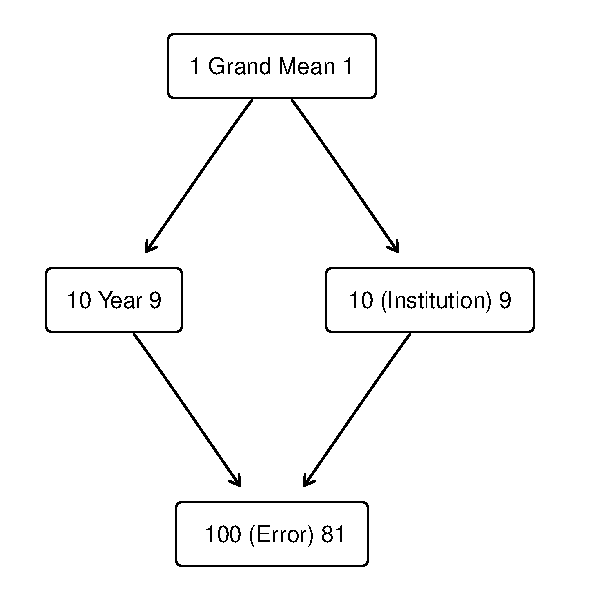
\includegraphics{Stat_461_Final_Project_Report_files/figure-latex/hasse-1} 

}

\caption{Hasse Diagram}\label{fig:hasse}
\end{figure}

As explained above, we will use ANOVA to conduct the analysis. After
analyzing the Hasse diagram found in Figure \ref{fig:hasse}, we decided
the best model to use for our study is a One Way Repeated Measures
(Within-Subjects) ANOVA Model. This method is effective because we can
observe if there are statistically significant differences in the sample
arithmetic means between each school year. This will also allow to
reduce the amount of subject-to-subject variation present within our
model by applying each ``year treatment'' to each individual
institution. If we were to find evidence to reject the null hypothesis
that there is no statistically significant difference between the sample
arithmetic means, we could then conduct post-hoc analysis to determine
if later years caused the proportion of women in STEM to increase. The
null and alternative hypothesis are formally expressed below.

INSERT HYPOTHESIS CORRECTLY

\subsubsection{Type I Error Rate}\label{type-i-error-rate}

We have decided that we will control Experimentwise Error Rate at 10\%
(\(\mathcal{E}_{I}=0.10\)) for both components of our study (ANOVA and
Logistic Regression portions). Given the low-stakes nature of our study,
we believed it was reasonable to use a more liberal Type I Error control
method. Having a Type I Error would not cause a significant impact nor
incur overwhelming costs, so having a low evidentiary requirement is
justified. The EER will be naturally controlled through the use of our
ANOVA F Test of our model. We also plan to set our unusualness threshold
at the same level as our Type I Error Rate (\emph{UT} = 0.10).

\subsection{Exploring the Data}\label{exploring-the-data}

\subsubsection{Attributes}\label{attributes}

There are two attributes we are concerned about in this study: the time
periods in which we are interested and the proportion of women pursuing
STEM. Because the question we are interested in is the change in the
proportion of women over time, graphing the data will provide some
general useful insights.

\begin{figure}
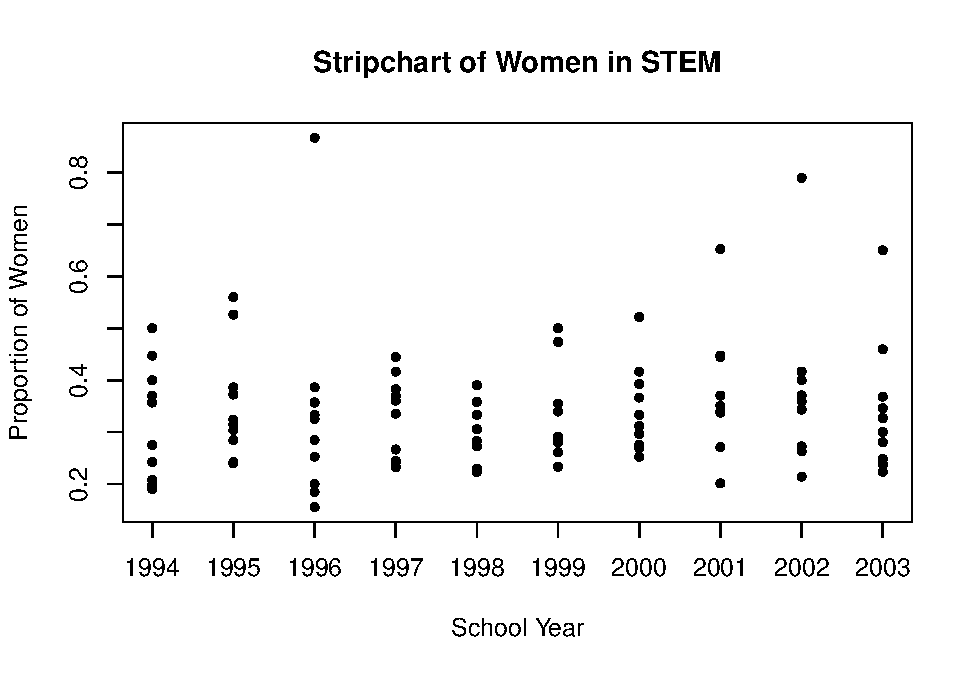
\includegraphics[width=.49\linewidth]{Stat_461_Final_Project_Report_files/figure-latex/strip-1} 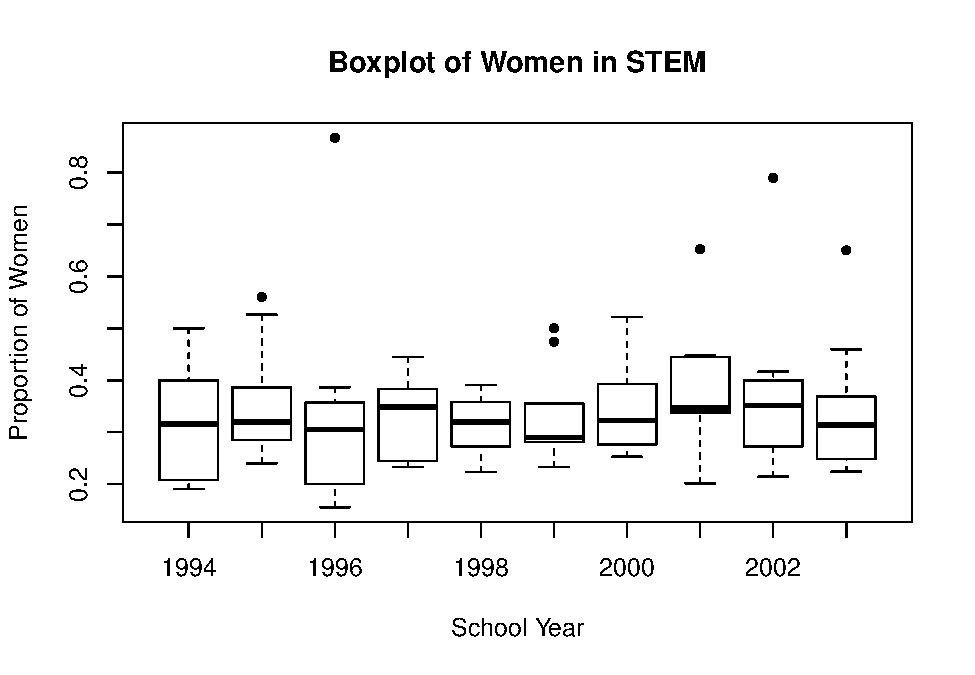
\includegraphics[width=.49\linewidth]{Stat_461_Final_Project_Report_files/figure-latex/strip-2} \caption{Stripchart and Boxplot of Proportion of Women over Time}\label{fig:strip}
\end{figure}

Figure \ref{fig:strip} gives plots of the data for all institutions over
the entire time period. Both plots appear to indicate that he majority
of institutions had a proportion of women between 0.2 -- 0.5. Given
that, it does not appear that there are any significant changes between
years. While it does look like there are some differences between years,
there is no clear upward/downward pattern that the data displays as the
years increase. This would suggest that as time went on, the proportion
of women in STEM had not increased significantly during the period of
1994 -- 2003 and that there are not statistically significant
differences in the sample arithmetic means between the years. ANOVA
analysis will provide greater insight into these details.

\begin{table}[H]

\caption{\label{tab:kabtab}Statistics for MIDFIELD Data}
\centering
\fontsize{9}{11}\selectfont
\begin{tabular}[t]{>{\centering\arraybackslash}p{0.3in}|>{\raggedleft\arraybackslash}p{0.7in}|>{\raggedleft\arraybackslash}p{0.25in}|>{\raggedleft\arraybackslash}p{0.8in}|>{\raggedleft\arraybackslash}p{0.25in}|>{\raggedleft\arraybackslash}p{0.7in}|>{\raggedleft\arraybackslash}p{0.4in}|>{\raggedleft\arraybackslash}p{0.4in}|>{\raggedleft\arraybackslash}p{0.8in}}
\hline
Year & Sample.Max & Q3 & Sample.Median & Q1 & Sample.Min & SAM & SAV & Sample.Skewness\\
\hline
1994 & 0.500 & 0.393 & 0.316 & 0.217 & 0.190 & 0.319 & 0.012 & 0.218\\
\hline
1995 & 0.560 & 0.383 & 0.319 & 0.290 & 0.240 & 0.355 & 0.012 & 0.753\\
\hline
1996 & 0.867 & 0.351 & 0.305 & 0.213 & 0.156 & 0.335 & 0.041 & 1.674\\
\hline
1997 & 0.444 & 0.379 & 0.348 & 0.250 & 0.233 & 0.330 & 0.006 & -0.003\\
\hline
1998 & 0.391 & 0.352 & 0.320 & 0.275 & 0.223 & 0.312 & 0.004 & -0.119\\
\hline
1999 & 0.500 & 0.351 & 0.290 & 0.282 & 0.233 & 0.331 & 0.008 & 0.859\\
\hline
2000 & 0.522 & 0.386 & 0.323 & 0.281 & 0.253 & 0.344 & 0.007 & 0.799\\
\hline
2001 & 0.652 & 0.426 & 0.346 & 0.338 & 0.201 & 0.375 & 0.015 & 0.860\\
\hline
2002 & 0.789 & 0.393 & 0.352 & 0.290 & 0.214 & 0.377 & 0.025 & 1.593\\
\hline
2003 & 0.650 & 0.363 & 0.314 & 0.257 & 0.224 & 0.344 & 0.016 & 1.223\\
\hline
\end{tabular}
\end{table}

Table 1 gives the values of various descriptive statistics for the
proportion of women pursuing STEM degrees by time periods. From the
table, we can observe that the sample arithmetic means range from 0.31
-- 0.38 which indicates that the means are very similar to each other.
The year with the lowest proportion of women in STEM is 1998 and the
year with the highest proportion is 2002. The sample arithmetic variance
is also very small across all the years. The sample skewness values vary
across the years which indicate that there may exist some outlier cases.
The graphs shown above outline some of the years with outlier cases.

\subsection{ANOVA Assumption Testing}\label{anova-assumption-testing}

In order to properly make use of our One Way Repeated Measures
(Within-Subjects) ANOVA Model, we must first check that our data passes
the proper assumption for such a model. These assumptions are the
normality of our residuals as well as our random effects,
homoscedasticity of our residuals, as well as a lack of interaction
between our subjects. Since we are also expecting a lack of independence
between our observations, we will be using Mauchly's test of Sphericity
to compensate for such violations. Upon checking the assumptions of our
original data, we noticed many issues regarding the normality and
homoscedasticity within the data, and decided to use a
log-transformation of our response variable in order to adjust to our
model
\footnote{An inclusion of the assumption visualizations for the original data along with a detailed explanation has been included within Appendix B}.

\clearpage

\subsubsection{Normality of Residuals and Random
Effects}\label{normality-of-residuals-and-random-effects}

\begin{figure}
\centering
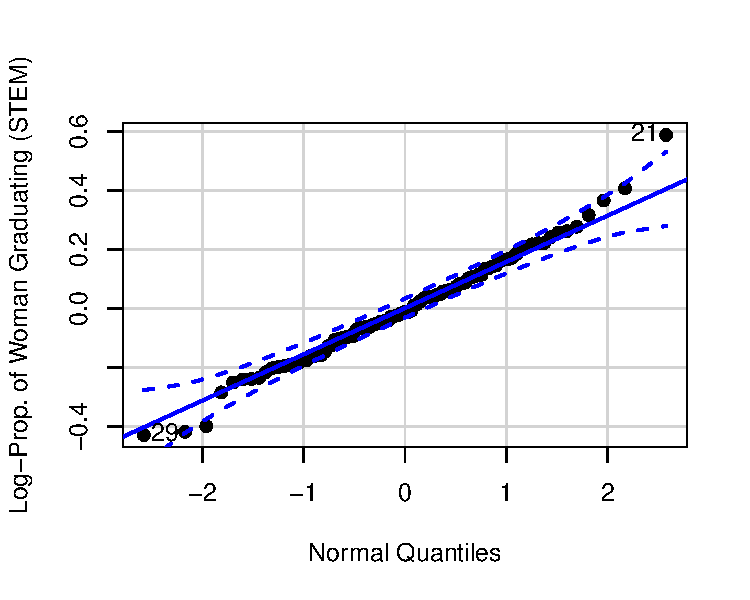
\includegraphics{Stat_461_Final_Project_Report_files/figure-latex/logNormality-1.pdf}
\caption{Normal Quantile Plot (Residuals) for Log-Transformed MIDFIELD
Data}
\end{figure}

Looking at the Normal Quantile Plot of the residuals for our
log-transormed data seen in Figure 3, we see that our residuals exist
mostly within our 90\% confidence envelope. There do appear to be a
couple of value either on the edge or just outside of the confidence
envelope, which could represent slight potential outliers within the
data. However, these values appear to deviate very slightly from a
normal distribution, thus we will assume that our residuals appear to be
normally distributed.

\begin{figure}
\centering
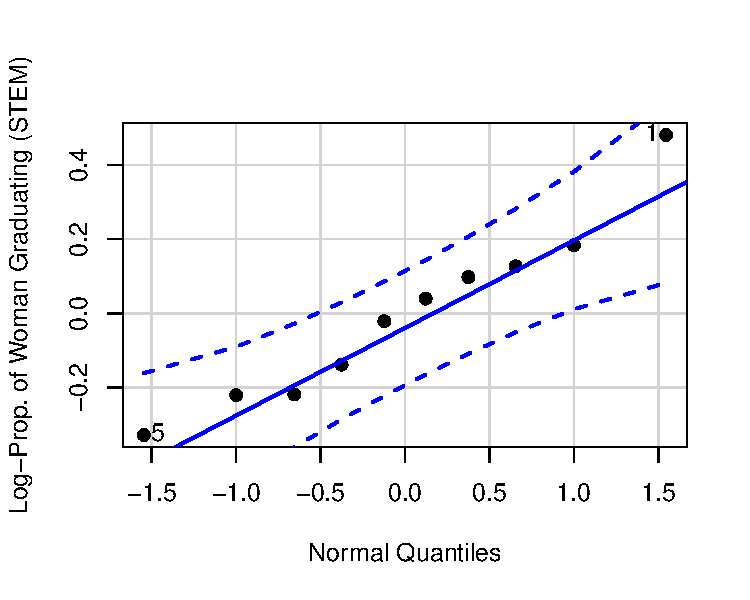
\includegraphics{Stat_461_Final_Project_Report_files/figure-latex/logNormalityRE-1.pdf}
\caption{Normal Quantile Plot (Random Effects) for Log-Transformed
MIDFIELD Data}
\end{figure}

Within Figure 4 above, we are given an visualization of the Normal
Quantile plot for our random effects (our institutions). Within the
plot, all values appear to be within the 90\% confidence envelope. There
appears to be no presence in potential outliers within the plot. Thus,
our random effects appear to be normally distributed, and we can assume
that normality of our residuals and random effects have been satisfied.

\subsubsection{Homoscedasticity of
Residuals}\label{homoscedasticity-of-residuals}

\begin{figure}
\centering
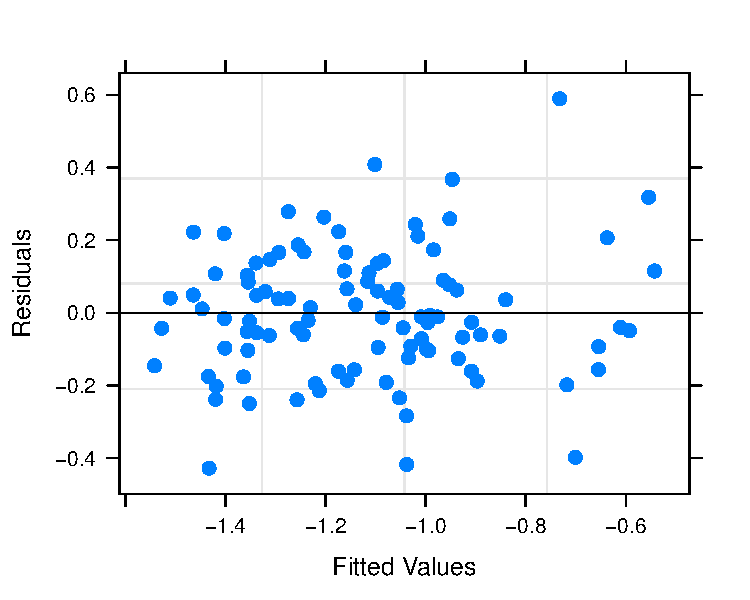
\includegraphics{Stat_461_Final_Project_Report_files/figure-latex/logHomoscedasticity-1.pdf}
\caption{Tukey-Anscombe Plot for Log-Transformed MIDFIELD Data}
\end{figure}

In order to interpret the homoscedasticity of our residuals, we turn to
the Tukey-Anscombe plot within Figure 5. Upon our initial analysis,
there appears to be no fanning present within our plot, which is a good
indicator that homoscedasticity is present. We can also roughly see that
their is no large difference in the vertical spread of our residuals.
Thus, we will decide that our assumption of normality has been
satisfied.

\subsubsection{Interaction}\label{interaction}

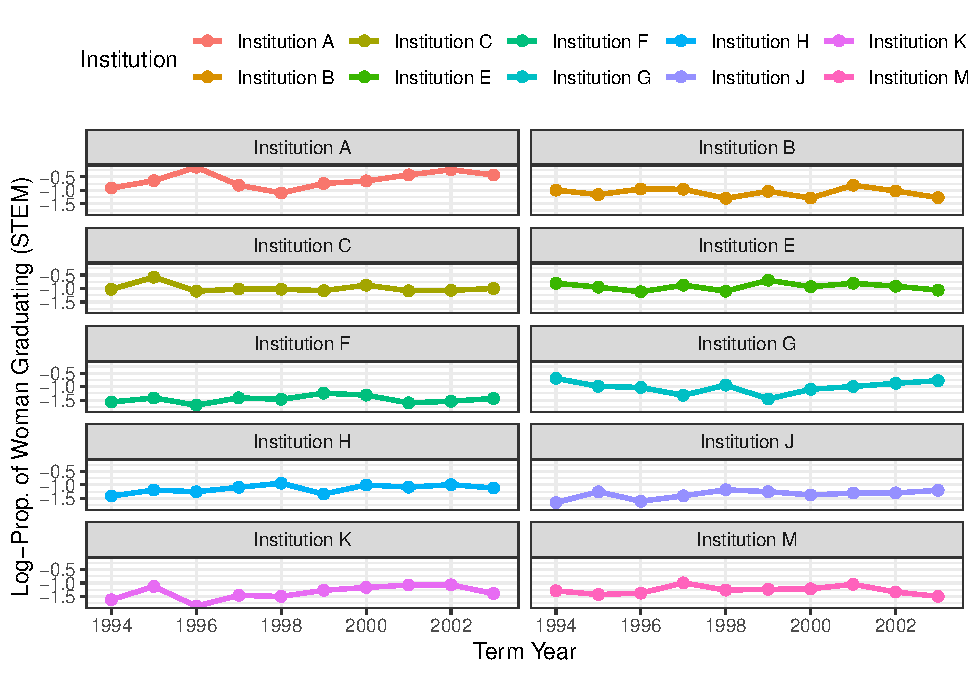
\includegraphics{Stat_461_Final_Project_Report_files/figure-latex/logInteraction-1.pdf}

In order to use our ANOVA model, we must check for a lack of interaction
between our subjects. Using the interaction plots above, we are given
the individual plots for the log-proportion of women graduating in STEM
by term year. Within the plot, we see potential interactions present
such as between the years 1995 and 1996 for institution's A and G.
However there appear to be few visual cues of interactions present, so
we will proceed with caution and assume that there is no interaction
present.

\subsubsection{Sphericity}\label{sphericity}

\begin{table}[H]

\caption{\label{tab:Sphericity}Mauchly's Test for Sphericity}
\centering
\fontsize{12}{14}\selectfont
\begin{tabular}[t]{l|c|c}
\hline
  & Test Statistic & p-value\\
\hline
Term\_Year & 0 & 0.019\\
\hline
\multicolumn{3}{l}{\textit{Note: } Computer rounding has made test statistic appear to be zero.}\\
\end{tabular}
\end{table}

Lastly, we will be using the results from Mauchly's test of Sphericity
in order to determine if our repeated measures are compoundly
symmetrical. Upon analysis of Table 2 above, we see that we acheived a
\emph{p}-value of 0.019. Comparing our p-value to our Type I Error Rate
of 0.1, we determine that our p-value is much less than our error rate.
THus, we will decide that our data violates the assumption of
sphericity. We will proceed with our omnibus testing, however we will
include adjustments methods to combat our violation of sphericity.

\subsection{Omnibus Results}\label{omnibus-results}

\begin{table}[H]

\caption{\label{tab:univariate Results}ANOVA Table Within-Subjects: Log of Proportion of Women Graduating in STEM}
\centering
\fontsize{12}{14}\selectfont
\begin{tabular}[t]{l|c|c|c|c|c|c}
\hline
  & Numerator DF & Denominator DF & Term SS & Error SS & F Ratio & p-value\\
\hline
(Intercept) & 1 & 9 & 125.639 & 5.820 & 194.279 & 0.000\\
\hline
Term\_Year & 9 & 81 & 0.386 & 3.011 & 1.155 & 0.335\\
\hline
\multicolumn{7}{l}{\textit{Note: } Computer rounding has made the p-values look like zero.}\\
\end{tabular}
\end{table}

Looking at the results or our Repeated Measures ANOVA Model above in
Table 3, we see that our term year achieved an \emph{F} Ratio of 1.155.
In other words, our term year factor accounts for around 1.15 times the
variation as our error term. We would most likely expect to achieve an F
Ratio such as this 33\% (\emph{p}-value = 0.335) of time under our
model's null hypothesis, which is a considerable amount of time.
Comparing our \emph{p}-value with our unusualness threshold (\emph{UT} =
0.10), we can see that our \emph{p}-value is not less than our
threshold, which in turn would result in the decision of failing to
reject our model's null hypothesis. However, due to the issues with
sphericity that we noted earlier, we must adjust our model to account
for our violations.

\begin{table}[H]

\caption{\label{tab:sphericityAdjustments}Adjustments for Sphericity Violations}
\centering
\fontsize{12}{14}\selectfont
\begin{tabular}[t]{l|c|c|c|c}
\hline
  & Greenhouse-Geiser & p-value & Huynh-Feldt & p-value\\
\hline
Term\_Year & 0.498 & 0.347 & 1.052 & 0.335\\
\hline
\multicolumn{5}{l}{\textit{Note: } Huynh-Feldt eps is being treated as 1.}\\
\end{tabular}
\end{table}

In order to handle our violations of sphericity, we look upon the
Greenhouse-Geiser and Huynh-Feldt adjustments of our \emph{p}-value.
Table 4 provides us with these adjustments. Our p-values using
Greenhouse-Geiser and Huynh-Feldt adjustments are 0.347 and 0.335,
respectively. Even when we use these adjusted \emph{p}-values, we still
see that our \emph{p}-values are much greater than our unusualness
threshold (\emph{UT} = 0.10). Thus, we will fail to reject our null
hypothesis and continue to act as if there is no significant difference
in the log proportion of women graduating with STEM degrees in our
collection of institutions due to the term year. In other words, we
interpret that there is not a significant increase or decrease in the
proportion of women graduating in STEM fields throughout our selected
time period.

\section{Exploring the Effect of Race and Gender on Drop Out Rates after
Introductory
Calculus}\label{exploring-the-effect-of-race-and-gender-on-drop-out-rates-after-introductory-calculus}

The second portion to our analysis considers the role of the
introductory calculus course as a weed out course for STEM majors.
Introductory calculus is a requirement for nearly all STEM majors and is
one of the most commonly cited reasons for students to leave the STEM
major. \cite{paper} While works such as that done by Rasmussen and Ellis
have considered factors impacting the probability of continuing the
calculus curriculum after the first calculus course, we wish to consider
factors that impact students' probability of leaving the STEM major
after introductory calculus, in particular to see how the probability
varies by race and gender.

To consider this problem, we use the MIDFIELD data to identify STEM
students who took Calculus I and label them as either having dropped out
of the STEM field in association with Calculus I or not having dropped
out of the STEM field in association with introductory
calculus.\footnote{A more detailed description of the data wrangling techniques and the methods by which the drop out variable was created can be found in Appendix A.}
We then develop a logistic regression model to model each students'
probability of dropping out after introductory calculus based on their
race and gender in order to test our hypothesis that at least one of
race and gender affect a student's probability of dropping out of the
STEM program after introductory calculus against the null hypothesis
that neither is a significant factor.

\subsection{Exploratory Analysis}\label{exploratory-analysis}

\begin{figure}
\centering
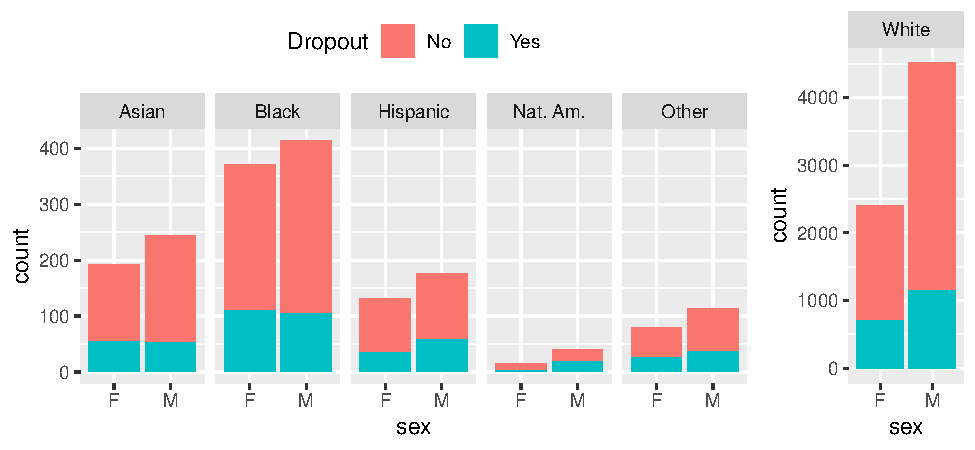
\includegraphics{Stat_461_Final_Project_Report_files/figure-latex/comboplots-1.pdf}
\caption{Dropouts by race and gender}
\end{figure}

We begin by visualizing the collected dropout data as seen in Figure 6.
We see that we are treating gender as a factor, for which we will assume
only two levels. Race is also a factor, which we will treat as having
six levels: White, Asian, Black, Hispanic, Native American, and Other
Minorities. Note that the other minority group also contains the
category international, which was included in the MIDFIELD dataset but
regrouped to other minorities for this analysis. It is also worth
considering the wide variety in sample size between the different
categories, with White having an overwhelming majority and Native
American having only barely enough to be considered as an individual
category.

Considering this visualization relative to our subject, we see that
females and several minority groups appear to be overall
underrepresented in this data. Females also appear to generally have
higher numbers of dropouts relative to population size for most races.

\subsection{Assumption Testing}\label{assumption-testing}

Logistic regression requires five assumptions to be satisfied:
appropriate outcome structure, independence of observations, absence of
multicollinearity, linearity of independent vars and log odds, and
sufficiently large sample size. \cite{glmassumptions} The first and last
of these are clearly met as we designed the dependent variable to be
binary and the size of the sample considered is over 8,000
students.\footnote{The full MIDFIELD dataset contains over 97,000 students. The smaller number used in the analysis is a result of filtering the students to STEM students who were identified as having taken an introductory calculus course.}
We do conceed, however,that some individual groups, such as female
native americans, do have a somewhat small sample size within this large
group, so this conclusions drawn for such groups must be closely
ridiculed.

Considering the linearity of independent variables relative to log odds,
we compare the dropout rate of each individual group in the below plot.

\begin{figure}
\centering
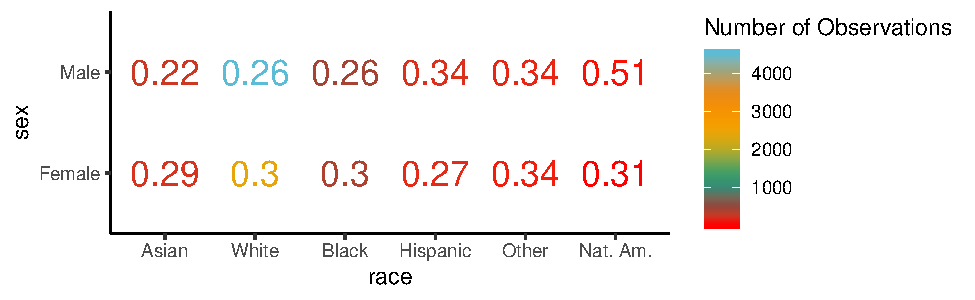
\includegraphics{Stat_461_Final_Project_Report_files/figure-latex/secondplot-1.pdf}
\caption{Dropout rates compared by race and gender}
\end{figure}

We see that for the three largest racial groups females have higher
dropout rates than males with other minorities as equal and the last two
categories having the reverse trend. Likewise, for most pairs of races,
similarities and differences in proportion dropping increase or decrease
consistently for males and females with the Hispanic and Native American
groups again providing the only mild exceptions, for example comparing
either to the Other Minorities category. This implies that there could
be some mild issues with the assumption of the independent variables'
linearity with log odds. We will, however, still proceed with the
analysis noting that these mild issues primarily occur among the least
common groups in the population and that any results of the analysis
pertaining to these smaller groups will need to be done
cautiously.\footnote{Particularly considering the smaller sample size in the Native American and to a lesser extent Hispanic groups, it may seem reasonable to merge one or both of these groups into the Other Minorities category. A condensed summary of the analysis making both of these choices is shown in Appendix C.}

To consider multicollinearity, we can use the variance inflation factor
(vif). The calculated values for vif were 1.009 for each predictor,
which is less than 4, the commonly used indicator of collinearity
problems. Therefore, we may proceed under the assumption that this
assumption holds.

The last assumption, and most tricky to consider, is the independence of
observations. While each student's measurements are taken individually
without regard to any other student in the study, our data does not give
any way for us to know that students, particularly in the same
institution at the same time period, interact with or influence each
other in a meaningful way. However, it is reasonable to assume that if
these influences exist, they would be negligible, particularly
considering that we are considering students' choices in educational
field which would rarely be impacted by infuences from the choices of
the other student.

Therefore, aside from a small linearity issue that we will continue to
acknowledge, we decide that all of our assumptions have been
sufficiently met, so we may proceed with our analysis.

\subsection{Developing the Model}\label{developing-the-model}

In developing the logistic regression model, we will use a baseline of a
white male. The resulting model is shown in the below table.

\begin{table}[H]

\caption{\label{tab:odds_ratios}Odds Ratios Relative to white men}
\centering
\fontsize{12}{14}\selectfont
\begin{tabular}[t]{l|l|c}
\hline
  & Odds Ratio & P-value\\
\hline
Female & 1.217 & 0.000\\
\hline
Asian & 0.888 & 0.298\\
\hline
Black & 1.012 & 0.883\\
\hline
Hispanic & 1.196 & 0.157\\
\hline
Native American & 2.283 & 0.002\\
\hline
Other Minorities & 1.356 & 0.049\\
\hline
\end{tabular}
\end{table}

Based on our test and the p values it produced, the only significant
terms are gender, the Native American race, and Other Minority races.
The p value for the impact of race rounds to 0 in the table, implying
that assuming the null hypothesis we would expect to see results at
least as extreme as we did nearly none of the time. Similarly, for the
Native American group, we would expect to see results this extreme only
.2\% of the time and for the other minority groups we would expect to
see a value this extreme only 4.9\% of the time. Their odds ratios,
which are set using the white man as a baseline, then tell us how much
more likely these students are to drop out. For example, a randomly
selected female is predicted to be 1.217 times more likely to drop out
than randomly selected male from the population and a randomly selected
Native American is predicted to be over twice as likely to drop out
after introductory calculus compared to a randomly selected White
student. This tells us that our data suggests that gender does influence
the impact of introductory calculus as a weed out course with
significance. Race, however, only statistically significantly affects
the dropout rate after calculus 1 for students of Native American
heritage and those from races that did not fall into any of the given
categories. We should point out, however, that the Native American group
was the smallest group, containing only approximately 60 total students,
and contained some assumption issues, so the result should be taken with
caution. Similarly the group of Other Minorities, most likely contains a
rather diverse group of students and therefore is difficult to interpret
entirely on its own. Similarly, recall that the groups Hispanic and
Native American followed a slightly different pattern in our assumptions
check, so we must be cautious on assertions we make about these groups,
both in the effects of race and gender. Note, however, that the results
remain consistent even when these groups are merged into the Other
category, the results of which are shown in Appendix C.

We can also view the predicted probability of dropping out by race and
gender in the below table.

\begin{table}[H]

\caption{\label{tab:pred}Prediction of Drop Out Probability by Race and Gender}
\centering
\fontsize{12}{14}\selectfont
\begin{tabular}[t]{l|c|c|c|c|c|c}
\hline
  & White & Asian & Black & Hispanic & Native Americans & Other Minorities\\
\hline
Male & 0.258 & 0.236 & 0.26 & 0.294 & 0.442 & 0.320\\
\hline
Female & 0.297 & 0.273 & 0.30 & 0.336 & 0.491 & 0.365\\
\hline
\end{tabular}
\end{table}

These predictions show a similar story where the females are predicted
to be more likely to drop out than the men and Native Americans and
Other Minorities have the largest predicted dropout rates among the
different races.

We should also consider the effect size of the model. The below table
gives the values for McFadden's, Coxsnell's, and Nagelkerke's
pseudo-R\(^2\) statistics.

\begin{table}[H]

\caption{\label{tab:efntable}Effect Sizes for the Effects of Race and Gender on Dropout Rate}
\centering
\fontsize{12}{14}\selectfont
\begin{tabular}[t]{r|r|r}
\hline
McFadden & CoxSnell & Nagelkerke\\
\hline
0.003 & 0.003 & 0.005\\
\hline
\end{tabular}
\end{table}

McFadden's and Coxsnell's statistics suggest that the model explains
.3\% of the variation while Nagelkerke's suggests that the model
explains .5\% of the variation. While this may seem like a very small
amount, keep in mind that we are attempting to predict dropout rates
based solely on race and gender. We would not expect, and certainly not
hope, that these factors would explain a large amount of variation in
dropout rates nor was that the intended purpose of our analysis. It is
also worth noting that using a likelihood ratio test and chi\(^2\)
statistic, we get a p value of less than .0001, which implies that our
model should still be considered statistically significant relative to
the null model.

\section{Discussion and Further
Study}\label{discussion-and-further-study}

From the MIDFIELD data, we have explored two aspects of minority
participation in the STEM field. The first area we explored was whether
there has been a growth of the proportion of women graduating with STEM
degrees. Through the omnibus results from our study, we found that there
was not a sufficient decrease or increase in the proportion of women
graduating with STEM degrees with our collection of data.

The second area we explored was how the probability of dropping out of
the STEM field after taking an introductory calculus course varied among
different races and genders. In this case, we found that females were
more likely to drop out after introductory calculus than males, and some
minority groups also had a significantly higher probability of dropping
out.

These analyses combine to suggest that these aspects of women and
minorities in STEM should be further studied and indicates continuing
underlying biases against them. That being said, both parts of this
analysis did suffer from some issues that arose from incomplete data,
and it should be kept in mind that even the most recent data in the
MIDFIELD study only includes up to 2017. We also acknowledge that the
original intent of the MIDFIELD study was to target engineering, which
could have impacted our results. We would suggest that more study on
these matters would be useful, especially to consider more recent data
that targets all of STEM instead of primarily targetting engineering. We
would also suggest further study into the patterns we found, in
particular to explore what factors may be impeding the movement to get
women more involved in the STEM field and the causation behind the more
adverse effect that calculus has on women in comparision to men as well
as on only select minority groups.

\newpage

\begin{thebibliography}{9}
\bibitem{data}
Richard Layton, Russell Long and Matthew Ohland
  (2019). midfielddata: Student Record Data for 98,000
  Undergraduates. R package version 0.1.0.
  https://github.com/MIDFIELDR/midfielddata

\bibitem{cip6}
National Center for Education Statistics. (n.d.).  Browse CIP Codes. Retrieved from https://nces.ed.gov/ipeds/cipcode/browse.aspx?y=55

\bibitem{paper}
Rasmussen, C., \& Ellis, J. (2013). Students who switch out of calculus and the reasons why they leave. In Martinez, M. \& Castro Superfine, A (Eds.). \textit{Proceedings of the 35th annual meeting of the North American Chapter of the International Group for the
Psychology of Mathematics Education} (pp. 457-464). Chicago, IL: University of Illinois at Chicago.

\bibitem{glmassumptions}
Schreiber-Gregory, D. (2018). PDF.

\bibitem{intro}
Ohland, Matthew W., and Russell A. Long. The Multiple-Institution Database for Investigating Engineering Longitudinal Development: an Experiential Case Study of Data Sharing and Reuse. Advances in Engineering Education, 2016, advances.asee.org/wp-content/uploads/vol05/issue02/Papers/AEE-18-Ohland.pdf.

\end{thebibliography}

\newpage

\section{Appendix A: Data Wrangling
Methods}\label{appendix-a-data-wrangling-methods}

Due to the extensiveness of the data wrangling necessary for this
project, we leave the description of the process to this appendix and
exclude the code generating the model ready data for either component of
the project from the Code Appendix. For scripts to generate the model
ready data, contact the authors of this work. The data released by the
MIDFIELD project was originally separated into four data tables, whose
names and descriptions as well as the pertinent data to this analysis
pulled from them can be found in the table below.

\begin{table}[H]

\caption{\label{tab:midtables}MIDFIELD Data Tables}
\centering
\fontsize{12}{14}\selectfont
\begin{tabular}[t]{>{\raggedright\arraybackslash}p{1.1in}|>{\centering\arraybackslash}p{2.5in}|>{\centering\arraybackslash}p{2.5in}}
\hline
Table & Purpose & UsefulData\\
\hline
midfieldterms & Shows the students' status by term & Program of study by term\\
\hline
midfieldcourses & Shows each instance of a student taking a class & Semester in which Calculus 1 was taken\\
\hline
midfieldstudents & Shows personal information about each student & Race and Gender of each student\\
\hline
midfielddegrees & Shows the end degree, or lack thereof, earned by each student & Students that earned STEM degrees\\
\hline
\end{tabular}
\end{table}

In order to properly combine this data for our analysis, there were
several major obsticals to overcome. The first consideration was
identifying the STEM programs in the data. This was done by translating
the six digit cip codes into a binary variable that identified the code
as either within STEM or not within STEM. \cite{cip6} This method was
used for both portions of the analysis.

\subsection{Analysis Specific to Women in
STEM}\label{analysis-specific-to-women-in-stem}

While finding the proportion of women STEM graduates by institution by
year was rather straightforward, there were a few modelling decisions
regarding the data. The first decision was to exclude all data that came
from a year and institution that graduated fewer than 10 STEM students
in the given year. This was done with the intention of helping to
improve the reliability of the data.

A challenge that was ran into was fitting the data into the One Way
Repeated Measures (Within-Subjects) ANOVA Model. Due to the result of
the data exclusion mentioned above. Our subjects for our study (the
individual institutions) no longer had a response value for every
treatment, making our blocks incomplete. To combat this issue, two
decisions were made. First, two institutions, institutions l and d, were
removed from the data due to the lack of response values from the
treatments. The second decision was to subset the Midfield data to
include response values from the time period of 1994-2003, rather than
the original time period of 1989-2016. This decision was reached to
include the largest set of consecutive years in which each institution
provided a proper response value, thus making the blocks complete.

\subsection{Analysis Specific to Dropout Rates after Calculus
1}\label{analysis-specific-to-dropout-rates-after-calculus-1}

The most complicated challenge that we faced was to identify which
semester the student took their first calculus course. This issue
primarily involves the midfieldcourses data table. There are two
identifiers for course in this table: course title and course code.
While the course title can rather clearly identify courses that could be
considered Calculus 1, only three institutions, institutions c, d, and
l, provided course titles in the data.

This leaves the course code as an identifier of course. These codes,
however, vary by institution and are not standardized to match to
particular courses. In order to approach this issue and allow more of
the data to be used, we began cross-referencing subsets of course codes
from particular institutions in order to attempt to match the anonymized
data to a particular institution or a particular coding key in order to
figure out which course code matches to Calculus 1. Note that in the
attempt to create this matching, we excluded math courses from the
matching set then ensured the predicted Calculus 1 course appeared in
the data set. The institutions that were identified using this method
were institutions a, b, e, h, j, and l. We were unable to identify the
remaining institutions, so they were excluded from the second part of
our analysis.

Another major considertation to make was how to define when a student
drops out of the STEM field in association with Calculus 1. Noting that
the data considers each year to contain six semesters, we defined a
student to have dropped out of the STEM field in association with
Calculus 1 if they do not graduate with a STEM degree and they do not
appear in a STEM program in the fourth, fifth, or sixth semesters
following the most recent taking of the course. Simply put, we sample
the time period between six months and a year after the course and see
whether or not the student is still in STEM. The consideration of
whether or not the graduate in STEM prevents the accidental elimination
of any student that gradutates immediately or shortly after Calculus 1
while the slight delay between the measurement era and the actual taking
of the course gives time for the student to choose to drop out or change
majors and for this change to be recorded.

\newpage

\section{Appendix B: Assumptions on Non-transformed
Data}\label{appendix-b-assumptions-on-non-transformed-data}

Upon performing our assumption testing for a One Way Repeated Measures
(Within-Subjects) ANOVA Model, we had noticed issues with the normality
and homoscedasticity of the original data. We have included the graphs
used to interpret the normality and homoscedasticity below.

\subsection{Normality}\label{normality}

\begin{figure}
\centering
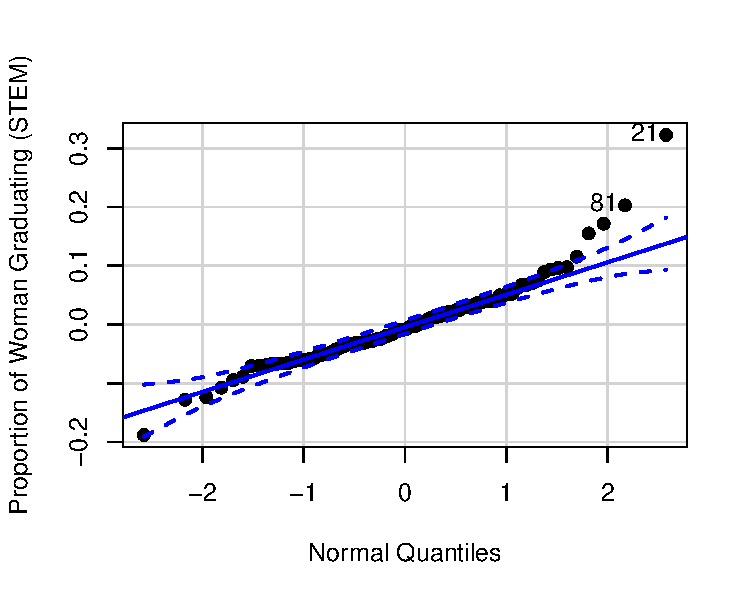
\includegraphics{Stat_461_Final_Project_Report_files/figure-latex/normality-1.pdf}
\caption{Normal Quantile Plot (Residuals) for Original MIDFIELD Data}
\end{figure}

Looking at the Normal Quantile Plot of the original data's residuals
above in Figure 7, We quickly notice a large positive skew in our
residuals. Due to the large amount of values existing outside of our
90\% confidence envelope, we can interpret that our residuals do not
appear to normally distributed. This lack of normality is a sign that a
potential transformation of the data would be sufficient.

\begin{figure}
\centering
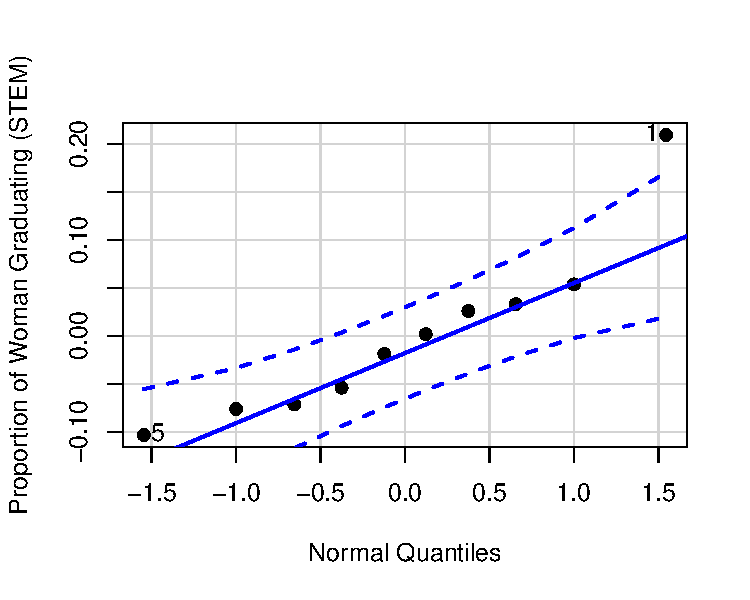
\includegraphics{Stat_461_Final_Project_Report_files/figure-latex/normalityRE-1.pdf}
\caption{Normal Quantile Plot (Random Effects) for Original MIDFIELD
Data}
\end{figure}

Upon analysis of the Normal Quantile plot for our original data's random
effects (see Figure 8 above), we see a potentially troublesome data
point within the plot. More specifically, there seems to a potential
outlier represented the the top right of our plot. Since this value is
outside of 90\% confidence envelope, we assume that the normality of our
random effects is not satisfied. Due to the lack of robustness within a
random effects model, even slight deviances to normality such as the one
we faced above can not be tolerated by the ANOVA model.

\subsection{Homoscedasticity}\label{homoscedasticity}

\begin{figure}
\centering
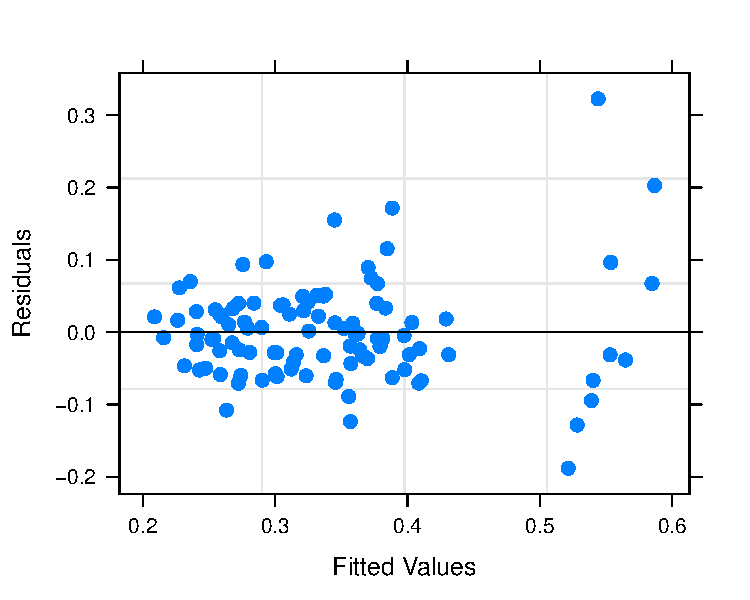
\includegraphics{Stat_461_Final_Project_Report_files/figure-latex/homoscedasticity-1.pdf}
\caption{Tukey-Anscombe Plot of Original MIDFIELD Data}
\end{figure}

Finally, we take a look at the Tukey-Anscombe plot in Figure 9 in order
to interpret our assumption of homoscedasticity. Looking at the plot, we
notice a fanning pattern present within our residuals. Due to the lack
of robustness within our model, we have decided to conclude that our
residuals appear to not be homoscedastic.

Due to all the issues present when checking the assumptions for our
model, we felt it neccessary to transform the original data. Upon
several trials with different transformations, we decided that a
log-transformation appeared to fit the most appropriately with our data.

\newpage

\section{Appendix C: Modified Logistic Regression
Models}\label{appendix-c-modified-logistic-regression-models}

In the assumption testing of our data, we recognized some issues with
the linearity of independent variables and log odds, the largest issue
considering the Native American group, which was also distinctly the
smallest group. It then makes sense to consider what happens when we
merge the Native American groups into the Other Minorities category.

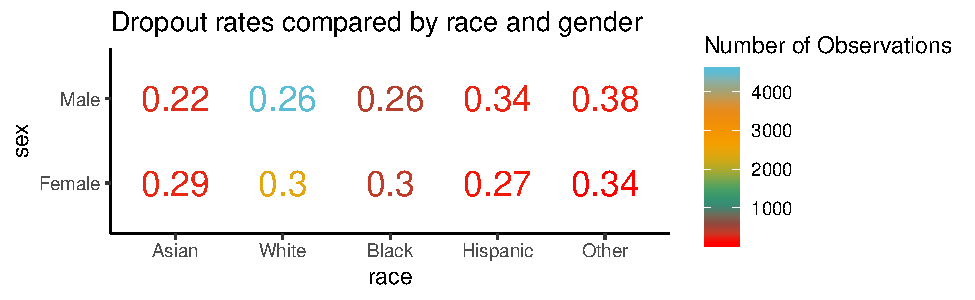
\includegraphics{Stat_461_Final_Project_Report_files/figure-latex/secondplot2-1.pdf}
As we could have predicted, the result still has some issues with the
Other Minorities and Hispanic categories in that they each have a higher
male proportion of female dropouts. The remainder of the analysis
remains similar.

The results are shown in the below table.

\begin{table}[H]

\caption{\label{tab:odds_ratios3}Odds Ratios Relative to white men}
\centering
\fontsize{12}{14}\selectfont
\begin{tabular}[t]{l|l|c}
\hline
  & Odds Ratio & P-value\\
\hline
Female & 0.907 & 0.000\\
\hline
Asian & 0.904 & 0.045\\
\hline
Black & 0.804 & 0.024\\
\hline
Hispanic & 0.916 & 0.252\\
\hline
Other Minorities & 1.082 & 0.458\\
\hline
\end{tabular}
\end{table}

Other than the Other Minorities category, which clearly changed in
composition, the odds ratios and p values are very similar to the
original analysis, which shows us that this decision is not overly
influential to our analysis and conclusions.

In an effort to better meet the linearity of independent observations
and log odds, we can also merge the Hispanic group into the Other
Minorities group.

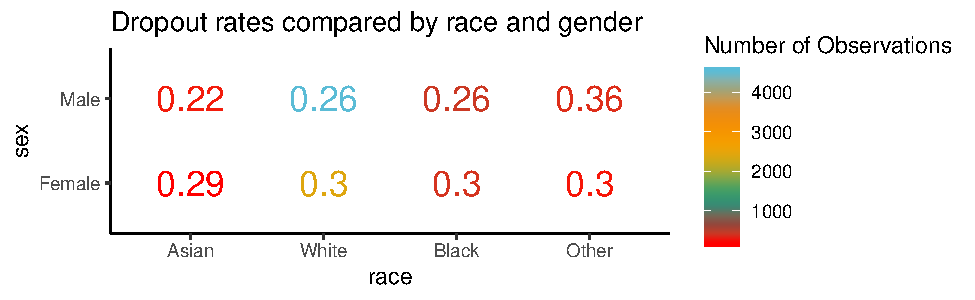
\includegraphics{Stat_461_Final_Project_Report_files/figure-latex/secondplot3-1.pdf}
Similar to the last case, the result is similar, with now only Other
Minorities presenting mild issues to our assumption. The rest of
analysis proceeds similarly with the test results shown below.

\begin{table}[H]

\caption{\label{tab:odds_ratios2}Odds Ratios Relative to white men}
\centering
\fontsize{12}{14}\selectfont
\begin{tabular}[t]{l|l|c}
\hline
  & Odds Ratio & P-value\\
\hline
Female & 0.908 & 0.000\\
\hline
Asian & 0.954 & 0.304\\
\hline
Black & 0.848 & 0.062\\
\hline
Other Minorities & 0.966 & 0.625\\
\hline
\end{tabular}
\end{table}

Other than the Other Minorities category, which clearly changed in
composition, the odds ratios and p values are still very similar to the
original analysis, so the decision is still relatively unimportant. That
being said, none of these models entirely meet assumptions, but the last
does come relatively close and produces a similar result to our original
model.

\newpage

\section{Appendix D: Code Appendix}\label{appendix-d-code-appendix}

\begin{Shaded}
\begin{Highlighting}[]
\KeywordTok{library}\NormalTok{(tidyr)}
\KeywordTok{library}\NormalTok{(dplyr)}
\KeywordTok{library}\NormalTok{(data.table)}
\KeywordTok{library}\NormalTok{(midfielddata)}
\KeywordTok{library}\NormalTok{(Metrics)}
\KeywordTok{library}\NormalTok{(caret)}
\KeywordTok{library}\NormalTok{(rcompanion)}
\KeywordTok{library}\NormalTok{(ggplot2)}
\KeywordTok{library}\NormalTok{(hasseDiagram)}
\KeywordTok{library}\NormalTok{(kableExtra)}
\KeywordTok{library}\NormalTok{(cowplot)}
\KeywordTok{library}\NormalTok{(wesanderson)}
\KeywordTok{library}\NormalTok{(magrittr)}
\KeywordTok{library}\NormalTok{(psych)}
\KeywordTok{suppressMessages}\NormalTok{(}\KeywordTok{library}\NormalTok{(car))}
\NormalTok{ALabs <-}\StringTok{ }\KeywordTok{c}\NormalTok{(}\StringTok{"1 Grand Mean 1"}\NormalTok{, }\StringTok{"10 Year 9"}\NormalTok{,}
              \StringTok{"10 (Institution) 9"}\NormalTok{, }\StringTok{" 100 (Error) 81"}\NormalTok{)}
\NormalTok{AMat <-}\StringTok{ }\KeywordTok{matrix}\NormalTok{(}\DataTypeTok{data =}\NormalTok{ F, }\DataTypeTok{nrow =} \DecValTok{4}\NormalTok{, }\DataTypeTok{ncol =} \DecValTok{4}\NormalTok{)}
\NormalTok{AMat[}\DecValTok{1}\NormalTok{, }\KeywordTok{c}\NormalTok{(}\DecValTok{2}\OperatorTok{:}\DecValTok{4}\NormalTok{)] =}\StringTok{ }\NormalTok{AMat[}\KeywordTok{c}\NormalTok{(}\DecValTok{2}\OperatorTok{:}\DecValTok{3}\NormalTok{), }\DecValTok{4}\NormalTok{] =}\StringTok{ }\NormalTok{T}
\NormalTok{hasseDiagram}\OperatorTok{::}\KeywordTok{hasse}\NormalTok{(AMat, ALabs)}
\NormalTok{m_f<-}\KeywordTok{read.csv}\NormalTok{(}\StringTok{"~/master_anova.csv"}\NormalTok{)}
\NormalTok{m_f}\OperatorTok{$}\NormalTok{term_degree<-}\KeywordTok{as.factor}\NormalTok{(m_f}\OperatorTok{$}\NormalTok{term_degree)}
\NormalTok{m_f}\OperatorTok{$}\NormalTok{institution<-}\KeywordTok{as.factor}\NormalTok{(m_f}\OperatorTok{$}\NormalTok{institution)}
\NormalTok{tpx <-}\StringTok{ }\NormalTok{m_f[,}\DecValTok{1}\NormalTok{]}
\NormalTok{tpx}
\NormalTok{instx <-}\StringTok{ }\NormalTok{m_f[,}\DecValTok{2}\NormalTok{]}
\NormalTok{px <-}\StringTok{ }\NormalTok{m_f[,}\DecValTok{3}\NormalTok{]}
\NormalTok{dfx <-}\StringTok{ }\KeywordTok{data.frame}\NormalTok{(tpx,instx, px)}
\NormalTok{dfx}

\NormalTok{df <-}\StringTok{ }\NormalTok{dfx[}\OperatorTok{-}\KeywordTok{c}\NormalTok{((}\KeywordTok{seq}\NormalTok{(}\DecValTok{1}\NormalTok{,}\DecValTok{31}\NormalTok{, }\DataTypeTok{by=}\DecValTok{1}\NormalTok{)), }\KeywordTok{seq}\NormalTok{(}\DecValTok{132}\NormalTok{,}\DecValTok{163}\NormalTok{, }\DataTypeTok{by=}\DecValTok{1}\NormalTok{)),]}
\NormalTok{df}
\KeywordTok{row.names}\NormalTok{(df) <-}\StringTok{ }\DecValTok{1}\OperatorTok{:}\KeywordTok{nrow}\NormalTok{(df)}

\NormalTok{tp2 <-}\StringTok{ }\NormalTok{df[,}\DecValTok{1}\NormalTok{]}
\NormalTok{tp <-}\StringTok{ }\KeywordTok{droplevels}\NormalTok{(tp2, }\DataTypeTok{exclude =} \ControlFlowTok{if}\NormalTok{(}\KeywordTok{anyNA}\NormalTok{(}\KeywordTok{levels}\NormalTok{(tp2))) }\OtherTok{NULL} \ControlFlowTok{else} \OtherTok{NA}\NormalTok{)}
\NormalTok{inst2 <-}\StringTok{ }\NormalTok{df[,}\DecValTok{2}\NormalTok{]}
\NormalTok{inst <-}\StringTok{ }\KeywordTok{droplevels}\NormalTok{(inst2, }\DataTypeTok{exclude =} \ControlFlowTok{if}\NormalTok{(}\KeywordTok{anyNA}\NormalTok{(}\KeywordTok{levels}\NormalTok{(inst2))) }\OtherTok{NULL} \ControlFlowTok{else} \OtherTok{NA}\NormalTok{)}
\NormalTok{p <-}\StringTok{ }\NormalTok{df[,}\DecValTok{3}\NormalTok{]}
\NormalTok{df2 <-}\StringTok{ }\KeywordTok{data.frame}\NormalTok{(tp,inst,p)}
\NormalTok{df2}\OperatorTok{$}\NormalTok{tp <-}\StringTok{ }\KeywordTok{as.factor}\NormalTok{(df2}\OperatorTok{$}\NormalTok{tp)}
\NormalTok{df2}\OperatorTok{$}\NormalTok{inst <-}\StringTok{ }\KeywordTok{as.factor}\NormalTok{(df2}\OperatorTok{$}\NormalTok{inst)}
\KeywordTok{stripchart}\NormalTok{(p}\OperatorTok{~}\NormalTok{tp, }\DataTypeTok{vertical =} \OtherTok{TRUE}\NormalTok{, }
           \DataTypeTok{pch =} \DecValTok{20}\NormalTok{, }\DataTypeTok{ylab =} \StringTok{"Proportion of Women"}\NormalTok{, }
           \DataTypeTok{xlab =} \StringTok{"School Year"}\NormalTok{, }
           \DataTypeTok{main =} \StringTok{"Stripchart of Women in STEM"}\NormalTok{)}

\KeywordTok{boxplot}\NormalTok{(p}\OperatorTok{~}\NormalTok{tp, }
        \DataTypeTok{pch =} \DecValTok{20}\NormalTok{, }\DataTypeTok{ylab =} 
        \StringTok{"Proportion of Women"}\NormalTok{, }
        \DataTypeTok{xlab =} \StringTok{"School Year"}\NormalTok{, }
        \DataTypeTok{main =} \StringTok{"Boxplot of Women in STEM"}\NormalTok{)}
\CommentTok{#getStats <- function(df2)}

\NormalTok{A <-}\StringTok{ }\NormalTok{psych}\OperatorTok{::}\KeywordTok{describeBy}\NormalTok{(}
  \DataTypeTok{x =} \KeywordTok{as.numeric}\NormalTok{(df2}\OperatorTok{$}\NormalTok{p), }\DataTypeTok{group =}\NormalTok{ df2}\OperatorTok{$}\NormalTok{tp, }
  \DataTypeTok{na.rm =} \OtherTok{TRUE}\NormalTok{, }\DataTypeTok{interp =} \OtherTok{TRUE}\NormalTok{, }
  \DataTypeTok{quant=} \KeywordTok{c}\NormalTok{(}\FloatTok{0.25}\NormalTok{,}\FloatTok{0.75}\NormalTok{), }\DataTypeTok{skew =} \OtherTok{TRUE}\NormalTok{, }
  \DataTypeTok{digits =} \DecValTok{3}\NormalTok{, }\DataTypeTok{mat =} \OtherTok{TRUE}\NormalTok{)}
\NormalTok{B <-}\StringTok{ }\KeywordTok{data.frame}\NormalTok{(}
  \DataTypeTok{Year =}\NormalTok{ A}\OperatorTok{$}\NormalTok{group1, }
  \DataTypeTok{Sample.Max =}\NormalTok{ A}\OperatorTok{$}\NormalTok{max, }
  \DataTypeTok{Q3=}\NormalTok{ A}\OperatorTok{$}\NormalTok{Q0.}\DecValTok{75}\NormalTok{, }
  \DataTypeTok{Sample.Median =}\NormalTok{ A}\OperatorTok{$}\NormalTok{median, }
  \DataTypeTok{Q1 =}\NormalTok{ A}\OperatorTok{$}\NormalTok{Q0.}\DecValTok{25}\NormalTok{, }
  \DataTypeTok{Sample.Min =}\NormalTok{ A}\OperatorTok{$}\NormalTok{min, }
  \DataTypeTok{SAM =}\NormalTok{ A}\OperatorTok{$}\NormalTok{mean, }
  \DataTypeTok{SAV =} \KeywordTok{round}\NormalTok{((A}\OperatorTok{$}\NormalTok{sd)}\OperatorTok{^}\DecValTok{2}\NormalTok{,}\DecValTok{3}\NormalTok{), }
  \DataTypeTok{Sample.Skewness =}\NormalTok{ A}\OperatorTok{$}\NormalTok{skew)}

\NormalTok{knitr}\OperatorTok{::}\KeywordTok{kable}\NormalTok{(B, }
             \DataTypeTok{caption =} \StringTok{"Statistics for MIDFIELD Data"}\NormalTok{,}
             \DataTypeTok{align =} \KeywordTok{c}\NormalTok{(}\StringTok{'c'}\NormalTok{, }\KeywordTok{rep}\NormalTok{(}\StringTok{'r'}\NormalTok{, }\DecValTok{9}\NormalTok{))) }\OperatorTok
\NormalTok{kableExtra}\OperatorTok{::}\KeywordTok{kable_styling}\NormalTok{(}\DataTypeTok{bootstrap_options =} \KeywordTok{c}\NormalTok{(}\StringTok{"striped"}\NormalTok{, }\StringTok{"condensed"}\NormalTok{),}
                          \DataTypeTok{font_size =} \DecValTok{9}\NormalTok{, }\DataTypeTok{latex_options =} \StringTok{"HOLD_position"}\NormalTok{)}\OperatorTok\StringTok{ }
\StringTok{  }\KeywordTok{column_spec}\NormalTok{(}\DecValTok{1}\NormalTok{, }\DataTypeTok{width =} \StringTok{'0.3in'}\NormalTok{) }\OperatorTok
\StringTok{  }\KeywordTok{column_spec}\NormalTok{(}\DecValTok{2}\NormalTok{, }\DataTypeTok{width =} \StringTok{"0.7in"}\NormalTok{)}\OperatorTok
\StringTok{  }\KeywordTok{column_spec}\NormalTok{(}\DecValTok{3}\NormalTok{, }\DataTypeTok{width =} \StringTok{"0.25in"}\NormalTok{)}\OperatorTok
\StringTok{  }\KeywordTok{column_spec}\NormalTok{(}\DecValTok{4}\NormalTok{, }\DataTypeTok{width =} \StringTok{"0.8in"}\NormalTok{)}\OperatorTok
\StringTok{  }\KeywordTok{column_spec}\NormalTok{(}\DecValTok{5}\NormalTok{, }\DataTypeTok{width =} \StringTok{"0.25in"}\NormalTok{)}\OperatorTok
\StringTok{  }\KeywordTok{column_spec}\NormalTok{(}\DecValTok{6}\NormalTok{, }\DataTypeTok{width =} \StringTok{"0.7in"}\NormalTok{)}\OperatorTok
\StringTok{  }\KeywordTok{column_spec}\NormalTok{(}\DecValTok{7}\NormalTok{, }\DataTypeTok{width =} \StringTok{"0.4in"}\NormalTok{)}\OperatorTok
\StringTok{  }\KeywordTok{column_spec}\NormalTok{(}\DecValTok{8}\NormalTok{, }\DataTypeTok{width =} \StringTok{"0.4in"}\NormalTok{)}\OperatorTok
\StringTok{  }\KeywordTok{column_spec}\NormalTok{(}\DecValTok{9}\NormalTok{, }\DataTypeTok{width =} \StringTok{"0.8in"}\NormalTok{)}
\NormalTok{df2}\OperatorTok{$}\NormalTok{logp <-}\StringTok{ }\KeywordTok{log}\NormalTok{(df2}\OperatorTok{$}\NormalTok{p)}
\NormalTok{midfieldLogM1 <-}\StringTok{ }\NormalTok{lme4}\OperatorTok{::}\KeywordTok{lmer}\NormalTok{(logp }\OperatorTok{~}\StringTok{ }\NormalTok{tp }\OperatorTok{+}\StringTok{ }\NormalTok{(}\DecValTok{1}\OperatorTok{|}\StringTok{ }\NormalTok{inst), }\DataTypeTok{data =}\NormalTok{ df2)}
\NormalTok{df2Wide <-}\StringTok{ }\NormalTok{tidyr}\OperatorTok{::}\KeywordTok{pivot_wider}\NormalTok{(df2,}\DataTypeTok{id_cols =}\NormalTok{ inst, }\DataTypeTok{names_from =}\NormalTok{ tp, }\DataTypeTok{values_from =}\NormalTok{ logp)}
\NormalTok{responseWide <-}\StringTok{ }\KeywordTok{as.matrix}\NormalTok{(df2Wide[ , }\DecValTok{2}\OperatorTok{:}\DecValTok{11}\NormalTok{])}
\NormalTok{midfieldMV <-}\StringTok{ }\KeywordTok{lm}\NormalTok{(responseWide }\OperatorTok{~}\StringTok{ }\DecValTok{1}\NormalTok{)}
\NormalTok{Term_Year <-}\StringTok{ }\KeywordTok{factor}\NormalTok{(}\KeywordTok{levels}\NormalTok{(df2}\OperatorTok{$}\NormalTok{tp))}

\NormalTok{### Create the table object}
\NormalTok{outputMV <-}\StringTok{ }\NormalTok{car}\OperatorTok{::}\KeywordTok{Anova}\NormalTok{(midfieldMV, }\DataTypeTok{idata =} \KeywordTok{data.frame}\NormalTok{(Term_Year),}
                   \DataTypeTok{idesign =} \OperatorTok{~}\NormalTok{Term_Year, }\DataTypeTok{type =} \StringTok{"III"}\NormalTok{)}
\NormalTok{midfieldMultivariate <-}\StringTok{ }\KeywordTok{summary}\NormalTok{(outputMV, }\DataTypeTok{multivariate=}\OtherTok{FALSE}\NormalTok{)}
\NormalTok{anovaFE <-}\StringTok{ }\NormalTok{car}\OperatorTok{::}\KeywordTok{qqPlot}\NormalTok{(}
  \DataTypeTok{x =} \KeywordTok{residuals}\NormalTok{(midfieldLogM1),}
  \DataTypeTok{distribution =} \StringTok{"norm"}\NormalTok{,}
  \DataTypeTok{envelope =} \FloatTok{0.90}\NormalTok{,}
  \DataTypeTok{xlab =} \StringTok{"Normal Quantiles"}\NormalTok{,}
  \DataTypeTok{ylab =} \StringTok{"Log-Prop. of Woman Graduating (STEM)"}\NormalTok{,}
  \DataTypeTok{pch =} \DecValTok{19}
\NormalTok{)}
\NormalTok{anovaRE <-}\StringTok{ }\NormalTok{car}\OperatorTok{::}\KeywordTok{qqPlot}\NormalTok{(}
  \DataTypeTok{x =}\NormalTok{ lme4}\OperatorTok{::}\KeywordTok{ranef}\NormalTok{(midfieldLogM1)}\OperatorTok{$}\NormalTok{inst[, }\StringTok{"(Intercept)"}\NormalTok{],}
  \DataTypeTok{distribution =} \StringTok{"norm"}\NormalTok{,}
  \DataTypeTok{envelope =} \FloatTok{0.90}\NormalTok{,}
  \DataTypeTok{xlab =} \StringTok{"Normal Quantiles"}\NormalTok{,}
  \DataTypeTok{ylab =} \StringTok{"Log-Prop. of Woman Graduating (STEM)"}\NormalTok{,}
  \DataTypeTok{pch =} \DecValTok{19}
\NormalTok{)}
\KeywordTok{plot}\NormalTok{(midfieldLogM1, }\DataTypeTok{which =} \DecValTok{1}\NormalTok{, }\DataTypeTok{pch =} \DecValTok{19}\NormalTok{, }\DataTypeTok{xlab =} \StringTok{"Fitted Values"}\NormalTok{, }\DataTypeTok{ylab =} \StringTok{"Residuals"}\NormalTok{)}
\KeywordTok{ggplot}\NormalTok{(}\DataTypeTok{data =}\NormalTok{ df2,}
  \DataTypeTok{mapping =} \KeywordTok{aes}\NormalTok{(}\DataTypeTok{x =}\NormalTok{ tp, }\DataTypeTok{y =}\NormalTok{ logp, }\DataTypeTok{color =}\NormalTok{ inst, }\DataTypeTok{group =}\NormalTok{ inst)) }\OperatorTok{+}
\StringTok{  }\KeywordTok{geom_point}\NormalTok{(}\DataTypeTok{size=}\DecValTok{2}\NormalTok{) }\OperatorTok{+}
\StringTok{  }\KeywordTok{geom_line}\NormalTok{(}\DataTypeTok{size=}\DecValTok{1}\NormalTok{) }\OperatorTok{+}
\StringTok{  }\KeywordTok{facet_wrap}\NormalTok{(}\OperatorTok{~}\StringTok{ }\NormalTok{inst, }\DataTypeTok{ncol =} \DecValTok{2}\NormalTok{) }\OperatorTok{+}
\StringTok{  }\KeywordTok{theme_bw}\NormalTok{() }\OperatorTok{+}
\StringTok{  }\KeywordTok{xlab}\NormalTok{(}\StringTok{"Term Year"}\NormalTok{) }\OperatorTok{+}
\StringTok{  }\KeywordTok{ylab}\NormalTok{(}\StringTok{"Log-Prop. of Woman Graduating (STEM)"}\NormalTok{) }\OperatorTok{+}
\StringTok{  }\KeywordTok{labs}\NormalTok{(}\DataTypeTok{color =} \StringTok{"Institution"}\NormalTok{) }\OperatorTok{+}
\StringTok{  }\KeywordTok{theme}\NormalTok{(}\DataTypeTok{legend.position=}\StringTok{"top"}\NormalTok{) }\OperatorTok{+}
\StringTok{  }\KeywordTok{scale_x_discrete}\NormalTok{(}\DataTypeTok{breaks=}\KeywordTok{seq}\NormalTok{(}\DecValTok{1994}\NormalTok{, }\DecValTok{2002}\NormalTok{, }\DecValTok{2}\NormalTok{))}

\KeywordTok{options}\NormalTok{(}\DataTypeTok{knitr.kable.NA=} \StringTok{""}\NormalTok{)}
\NormalTok{knitr}\OperatorTok{::}\KeywordTok{kable}\NormalTok{(}
  \KeywordTok{data.frame}\NormalTok{(}\KeywordTok{unclass}\NormalTok{(midfieldMultivariate}\OperatorTok{$}\NormalTok{sphericity.tests)),}
  \DataTypeTok{digits =} \DecValTok{3}\NormalTok{,}
  \DataTypeTok{col.names =} \KeywordTok{c}\NormalTok{(}\StringTok{"Test Statistic"}\NormalTok{, }\StringTok{"p-value"}\NormalTok{),}
  \DataTypeTok{caption =} \StringTok{"Mauchly's Test for Sphericity"}\NormalTok{,}
  \DataTypeTok{align =} \KeywordTok{c}\NormalTok{(}\StringTok{'c'}\NormalTok{,}\KeywordTok{rep}\NormalTok{(}\StringTok{'c'}\NormalTok{,}\DecValTok{2}\NormalTok{))}
\NormalTok{) }\OperatorTok
\StringTok{  }\NormalTok{kableExtra}\OperatorTok{::}\KeywordTok{kable_styling}\NormalTok{(}
    \DataTypeTok{bootstrap_options =} \KeywordTok{c}\NormalTok{(}\StringTok{"striped"}\NormalTok{, }\StringTok{"condensed"}\NormalTok{),}
    \DataTypeTok{font_size =} \DecValTok{12}\NormalTok{, }\DataTypeTok{latex_options =} \StringTok{"HOLD_position"}\NormalTok{) }\OperatorTok
\NormalTok{kableExtra}\OperatorTok{::}\KeywordTok{footnote}\NormalTok{(}
    \DataTypeTok{general =} \StringTok{"Computer rounding has made test statistic appear to be zero."}\NormalTok{,}
    \DataTypeTok{footnote_as_chunk =}\NormalTok{ T)}

\NormalTok{midfieldFrame <-}\StringTok{ }\KeywordTok{data.frame}\NormalTok{(}\KeywordTok{unclass}\NormalTok{(midfieldMultivariate}\OperatorTok{$}\NormalTok{univariate.tests))}
\NormalTok{midfieldFrame <-}\StringTok{ }\NormalTok{midfieldFrame[,}\KeywordTok{c}\NormalTok{(}\DecValTok{2}\NormalTok{,}\DecValTok{4}\NormalTok{,}\DecValTok{1}\NormalTok{,}\DecValTok{3}\NormalTok{,}\DecValTok{5}\NormalTok{,}\DecValTok{6}\NormalTok{)]}
\NormalTok{knitr}\OperatorTok{::}\KeywordTok{kable}\NormalTok{(}
\NormalTok{  midfieldFrame,}
  \DataTypeTok{digits =} \DecValTok{3}\NormalTok{,}
  \DataTypeTok{col.names =} \KeywordTok{c}\NormalTok{(}\StringTok{"Numerator DF"}\NormalTok{, }\StringTok{"Denominator DF"}\NormalTok{, }\StringTok{"Term SS"}\NormalTok{, }\StringTok{"Error SS"}\NormalTok{, }\StringTok{"F Ratio"}\NormalTok{, }\StringTok{"p-value"}\NormalTok{),}
  \DataTypeTok{caption =} \StringTok{"ANOVA Table Within-Subjects: Log of Proportion of Women Graduating in STEM"}\NormalTok{,}
  \DataTypeTok{align =} \KeywordTok{c}\NormalTok{(}\StringTok{'c'}\NormalTok{,}\KeywordTok{rep}\NormalTok{(}\StringTok{'c'}\NormalTok{,}\DecValTok{6}\NormalTok{))}
\NormalTok{) }\OperatorTok
\StringTok{  }\NormalTok{kableExtra}\OperatorTok{::}\KeywordTok{kable_styling}\NormalTok{(}
    \DataTypeTok{bootstrap_options =} \KeywordTok{c}\NormalTok{(}\StringTok{"striped"}\NormalTok{, }\StringTok{"condensed"}\NormalTok{),}
    \DataTypeTok{font_size =} \DecValTok{12}\NormalTok{, }\DataTypeTok{latex_options =} \StringTok{"HOLD_position"}\NormalTok{) }\OperatorTok
\StringTok{  }\NormalTok{kableExtra}\OperatorTok{::}\KeywordTok{footnote}\NormalTok{(}
    \DataTypeTok{general =} \StringTok{"Computer rounding has made the p-values look like zero."}\NormalTok{,}
    \DataTypeTok{footnote_as_chunk =}\NormalTok{ T)}
\NormalTok{knitr}\OperatorTok{::}\KeywordTok{kable}\NormalTok{(}
  \KeywordTok{data.frame}\NormalTok{(}\KeywordTok{unclass}\NormalTok{(midfieldMultivariate}\OperatorTok{$}\NormalTok{pval.adjustments)),}
  \DataTypeTok{digits =} \DecValTok{3}\NormalTok{,}
  \DataTypeTok{col.names =} \KeywordTok{c}\NormalTok{(}\StringTok{"Greenhouse-Geiser"}\NormalTok{, }\StringTok{"p-value"}\NormalTok{, }\StringTok{"Huynh-Feldt"}\NormalTok{, }\StringTok{"p-value"}\NormalTok{),}
  \DataTypeTok{caption =} \StringTok{"Adjustments for Sphericity Violations"}\NormalTok{,}
  \DataTypeTok{align =} \KeywordTok{c}\NormalTok{(}\StringTok{'c'}\NormalTok{,}\KeywordTok{rep}\NormalTok{(}\StringTok{'c'}\NormalTok{,}\DecValTok{4}\NormalTok{))}
\NormalTok{) }\OperatorTok
\StringTok{  }\NormalTok{kableExtra}\OperatorTok{::}\KeywordTok{kable_styling}\NormalTok{(}
    \DataTypeTok{bootstrap_options =} \KeywordTok{c}\NormalTok{(}\StringTok{"striped"}\NormalTok{, }\StringTok{"condensed"}\NormalTok{),}
    \DataTypeTok{font_size =} \DecValTok{12}\NormalTok{, }\DataTypeTok{latex_options =} \StringTok{"HOLD_position"}\NormalTok{) }\OperatorTok
\StringTok{  }\NormalTok{kableExtra}\OperatorTok{::}\KeywordTok{footnote}\NormalTok{(}
    \DataTypeTok{general =} \StringTok{"Huynh-Feldt eps is being treated as 1."}\NormalTok{,}
    \DataTypeTok{footnote_as_chunk =}\NormalTok{ T)}
\CommentTok{#Load data for logistic regression analysis}
\NormalTok{train<-}\KeywordTok{fread}\NormalTok{(}\StringTok{"~/master_glm.csv"}\NormalTok{) }\CommentTok{#Assumed location of data file}
\NormalTok{train<-train[race}\OperatorTok{!=}\StringTok{"Unknown"} \OperatorTok{&}\StringTok{ }\NormalTok{sex}\OperatorTok{!=}\StringTok{"Unknown"}\NormalTok{]}
\NormalTok{train<-train[,race}\OperatorTok{:}\ErrorTok{=}\KeywordTok{ifelse}\NormalTok{(race}\OperatorTok{==}\StringTok{"International"}\NormalTok{, }\StringTok{"Other"}\NormalTok{, race)]}

\CommentTok{# Create prep data for EDA plot}
\NormalTok{trainp<-train[,race}\OperatorTok{:}\ErrorTok{=}\KeywordTok{ifelse}\NormalTok{(race}\OperatorTok{==}\StringTok{"Native American"}\NormalTok{, }\StringTok{"Nat. Am."}\NormalTok{, race)]}
\NormalTok{trainp<-trainp[race}\OperatorTok{!=}\StringTok{"White"}\NormalTok{]}
\NormalTok{trainp<-trainp[,sex}\OperatorTok{:}\ErrorTok{=}\KeywordTok{ifelse}\NormalTok{(sex}\OperatorTok{==}\StringTok{"Male"}\NormalTok{, }\StringTok{"M"}\NormalTok{, }\StringTok{"F"}\NormalTok{)]}
\NormalTok{trainp<-trainp[,dropout}\OperatorTok{:}\ErrorTok{=}\KeywordTok{ifelse}\NormalTok{(dropout}\OperatorTok{==}\DecValTok{1}\NormalTok{, }\StringTok{"Yes"}\NormalTok{, }\StringTok{"No"}\NormalTok{)]}

\CommentTok{# Component of plot for minority groups}
\NormalTok{gg1<-}\KeywordTok{ggplot}\NormalTok{(}\DataTypeTok{data=}\NormalTok{trainp, }\KeywordTok{aes}\NormalTok{(}\DataTypeTok{x=}\NormalTok{sex, }\DataTypeTok{fill =} \KeywordTok{as.factor}\NormalTok{(dropout))) }\OperatorTok{+}\StringTok{  }
\StringTok{  }\KeywordTok{geom_bar}\NormalTok{() }\OperatorTok{+}\StringTok{ }
\StringTok{  }\KeywordTok{facet_grid}\NormalTok{ (}\OperatorTok{~}\NormalTok{race) }\OperatorTok{+}\StringTok{ }
\StringTok{  }\KeywordTok{theme}\NormalTok{(}\DataTypeTok{legend.position=}\StringTok{"top"}\NormalTok{) }\OperatorTok{+}\StringTok{ }
\StringTok{  }\KeywordTok{labs}\NormalTok{(}\DataTypeTok{fill=}\StringTok{"Dropout"}\NormalTok{) }

\CommentTok{# Component of plot for white group}
\NormalTok{trainp<-train[race}\OperatorTok{==}\StringTok{"White"}\NormalTok{]}
\NormalTok{trainp<-trainp[,sex}\OperatorTok{:}\ErrorTok{=}\KeywordTok{ifelse}\NormalTok{(sex}\OperatorTok{==}\StringTok{"Male"}\NormalTok{, }\StringTok{"M"}\NormalTok{, }\StringTok{"F"}\NormalTok{)]}
\NormalTok{gg2<-}\KeywordTok{ggplot}\NormalTok{(}\DataTypeTok{data=}\NormalTok{trainp, }\KeywordTok{aes}\NormalTok{(}\DataTypeTok{x=}\NormalTok{sex, }\DataTypeTok{fill =} \KeywordTok{as.factor}\NormalTok{(dropout))) }\OperatorTok{+}
\StringTok{  }\KeywordTok{geom_bar}\NormalTok{() }\OperatorTok{+}\StringTok{ }
\StringTok{  }\KeywordTok{facet_grid}\NormalTok{ (}\OperatorTok{~}\NormalTok{race) }\OperatorTok{+}\StringTok{ }
\StringTok{  }\KeywordTok{theme}\NormalTok{(}\DataTypeTok{legend.position =} \StringTok{"none"}\NormalTok{) }
\CommentTok{# Combine plots}
\KeywordTok{plot_grid}\NormalTok{(gg1, gg2, }\DataTypeTok{rel_widths =} \KeywordTok{c}\NormalTok{(}\FloatTok{3.5}\NormalTok{,}\DecValTok{1}\NormalTok{))}
\CommentTok{# Prep data for proportion grid plot}
\NormalTok{trainp2<-train}
\NormalTok{trainp2<-trainp2[,drop_rate}\OperatorTok{:}\ErrorTok{=}\KeywordTok{mean}\NormalTok{(dropout), keyby=}\KeywordTok{c}\NormalTok{(}\StringTok{"race"}\NormalTok{, }\StringTok{"sex"}\NormalTok{)]}
\NormalTok{trainp3<-train}
\NormalTok{trainp3<-trainp2[,n}\OperatorTok{:}\ErrorTok{=}\NormalTok{.N, keyby=}\KeywordTok{c}\NormalTok{(}\StringTok{"race"}\NormalTok{, }\StringTok{"sex"}\NormalTok{)]}
\NormalTok{trainp3}\OperatorTok{$}\NormalTok{race<-}\KeywordTok{factor}\NormalTok{(trainp2}\OperatorTok{$}\NormalTok{race, }
                     \DataTypeTok{levels=}\KeywordTok{c}\NormalTok{(}\StringTok{"Asian"}\NormalTok{, }\StringTok{"White"}\NormalTok{, }\StringTok{"Black"}\NormalTok{, }\StringTok{"Hispanic"}\NormalTok{, }\StringTok{"Other"}\NormalTok{, }\StringTok{"Nat. Am."}\NormalTok{))}

\CommentTok{# Make dropout proportion grid plot}
\KeywordTok{ggplot}\NormalTok{(}\KeywordTok{aes}\NormalTok{(}\DataTypeTok{x=}\NormalTok{race, }\DataTypeTok{y=}\NormalTok{sex, }\DataTypeTok{color=}\NormalTok{n), }\DataTypeTok{data=}\NormalTok{trainp3) }\OperatorTok{+}\StringTok{ }
\StringTok{  }\KeywordTok{geom_text}\NormalTok{(}\KeywordTok{aes}\NormalTok{(}\DataTypeTok{label=}\KeywordTok{round}\NormalTok{(drop_rate, }\DataTypeTok{digits=}\DecValTok{2}\NormalTok{)), }\DataTypeTok{size=}\DecValTok{6}\NormalTok{) }\OperatorTok{+}\StringTok{ }
\StringTok{  }\KeywordTok{scale_color_gradientn}\NormalTok{(}\DataTypeTok{colours =} \KeywordTok{wes_palette}\NormalTok{(}\StringTok{"Darjeeling1"}\NormalTok{, }\DecValTok{10}\NormalTok{, }\DataTypeTok{type =} \StringTok{"continuous"}\NormalTok{)) }\OperatorTok{+}
\StringTok{  }\KeywordTok{labs}\NormalTok{(}\DataTypeTok{color=}\StringTok{"Number of Observations"}\NormalTok{) }\OperatorTok{+}\StringTok{ }
\StringTok{  }\KeywordTok{theme_bw}\NormalTok{()}\OperatorTok{+}
\StringTok{  }\KeywordTok{theme}\NormalTok{(}\DataTypeTok{panel.border =} \KeywordTok{element_blank}\NormalTok{(), }\DataTypeTok{panel.grid.major =} \KeywordTok{element_blank}\NormalTok{(),}
\DataTypeTok{panel.grid.minor =} \KeywordTok{element_blank}\NormalTok{(), }\DataTypeTok{axis.line =} \KeywordTok{element_line}\NormalTok{(}\DataTypeTok{colour =} \StringTok{"black"}\NormalTok{))}
  
\CommentTok{# Correct training data to be ready for the rest of the analysis}
\NormalTok{train[,race}\OperatorTok{:}\ErrorTok{=}\KeywordTok{ifelse}\NormalTok{(race}\OperatorTok{==}\StringTok{"Nat. Am."}\NormalTok{,}\StringTok{"Native American"}\NormalTok{, race)]}
\NormalTok{train}\OperatorTok{$}\NormalTok{sex<-}\KeywordTok{as.factor}\NormalTok{(train}\OperatorTok{$}\NormalTok{sex)}
\NormalTok{train}\OperatorTok{$}\NormalTok{race<-}\KeywordTok{as.factor}\NormalTok{(train}\OperatorTok{$}\NormalTok{race)}

\CommentTok{# Set order for race and gender so that white men will be the baseline}
\NormalTok{Gender <-}\StringTok{ }\KeywordTok{factor}\NormalTok{(train}\OperatorTok{$}\NormalTok{sex, }\DataTypeTok{levels=}\KeywordTok{c}\NormalTok{(}\StringTok{'Male'}\NormalTok{, }\StringTok{'Female'}\NormalTok{))}
\NormalTok{Race<-}\KeywordTok{factor}\NormalTok{(train}\OperatorTok{$}\NormalTok{race, }
             \DataTypeTok{levels =} \KeywordTok{c}\NormalTok{(}\StringTok{"White"}\NormalTok{, }\StringTok{"Asian"}\NormalTok{, }\StringTok{"Black"}\NormalTok{, }\StringTok{"Hispanic"}\NormalTok{,}
                        \StringTok{"International"}\NormalTok{, }\StringTok{"Native American"}\NormalTok{, }\StringTok{"Other"}\NormalTok{))}
\NormalTok{glm_model<-}\KeywordTok{glm}\NormalTok{(dropout }\OperatorTok{~}\StringTok{ }\NormalTok{Gender }\OperatorTok{+}\StringTok{ }\NormalTok{Race, }\DataTypeTok{family =}\NormalTok{ binomial, }\DataTypeTok{data =}\NormalTok{ train)}

\CommentTok{# Check Multicollinearity}
\NormalTok{car}\OperatorTok{::}\KeywordTok{vif}\NormalTok{(glm_model)}

\CommentTok{# Calculate Odds Ratios}
\NormalTok{oddsrat <-}\StringTok{ }\KeywordTok{exp}\NormalTok{(parameters}\OperatorTok{::}\KeywordTok{model_parameters}\NormalTok{(glm_model)[}\DecValTok{2}\NormalTok{])}
\NormalTok{p <-}\StringTok{ }\NormalTok{parameters}\OperatorTok{::}\KeywordTok{model_parameters}\NormalTok{(glm_model)[}\StringTok{"p"}\NormalTok{]}
\NormalTok{dat <-}\StringTok{ }\KeywordTok{data.frame}\NormalTok{(}\DataTypeTok{Odds_Ratio=}\NormalTok{oddsrat, }\DataTypeTok{p=}\NormalTok{p)[}\OperatorTok{-}\DecValTok{1}\NormalTok{,]}
\KeywordTok{rownames}\NormalTok{(dat)<-}\KeywordTok{c}\NormalTok{(}\StringTok{"Female"}\NormalTok{, }\StringTok{"Asian"}\NormalTok{, }\StringTok{"Black"}\NormalTok{, }\StringTok{"Hispanic"}\NormalTok{, }\StringTok{"Native American"}\NormalTok{, }\StringTok{"Other Minorities"}\NormalTok{)}
\KeywordTok{setnames}\NormalTok{(dat, }\KeywordTok{c}\NormalTok{(}\StringTok{"Coefficient"}\NormalTok{, }\StringTok{"p"}\NormalTok{), }\KeywordTok{c}\NormalTok{(}\StringTok{"Odds Ratio"}\NormalTok{, }\StringTok{"P-value"}\NormalTok{))}

\CommentTok{# Table for Odds Ratios}
\NormalTok{knitr}\OperatorTok{::}\KeywordTok{kable}\NormalTok{(}
\NormalTok{  dat,}
  \DataTypeTok{digits =} \DecValTok{3}\NormalTok{,}
  \DataTypeTok{caption =} \StringTok{"Odds Ratios Relative to white men"}\NormalTok{,}
  \DataTypeTok{align =} \KeywordTok{c}\NormalTok{(}\StringTok{'l'}\NormalTok{,}\KeywordTok{rep}\NormalTok{(}\StringTok{'c'}\NormalTok{,}\DecValTok{4}\NormalTok{))}
\NormalTok{) }\OperatorTok
\StringTok{  }\NormalTok{kableExtra}\OperatorTok{::}\KeywordTok{kable_styling}\NormalTok{(}
    \DataTypeTok{bootstrap_options =} \KeywordTok{c}\NormalTok{(}\StringTok{"striped"}\NormalTok{, }\StringTok{"condensed"}\NormalTok{),}
    \DataTypeTok{font_size =} \DecValTok{12}\NormalTok{, }\DataTypeTok{latex_options =} \StringTok{"HOLD_position"}\NormalTok{)}

\CommentTok{# Get predictions for each combination of race and gender}
\NormalTok{test<-}\KeywordTok{data.table}\NormalTok{(}\DataTypeTok{Race =} \KeywordTok{c}\NormalTok{(}\StringTok{"White"}\NormalTok{, }\StringTok{"Asian"}\NormalTok{, }\StringTok{"Black"}\NormalTok{, }\StringTok{"Hispanic"}\NormalTok{, }\StringTok{"Native American"}\NormalTok{, }\StringTok{"Other"}\NormalTok{,}
                          \StringTok{"White"}\NormalTok{, }\StringTok{"Asian"}\NormalTok{, }\StringTok{"Black"}\NormalTok{, }\StringTok{"Hispanic"}\NormalTok{,  }\StringTok{"Native American"}\NormalTok{, }\StringTok{"Other"}\NormalTok{),}
                 \DataTypeTok{Gender=}\KeywordTok{c}\NormalTok{(}\StringTok{"Male"}\NormalTok{,}\StringTok{"Male"}\NormalTok{,}\StringTok{"Male"}\NormalTok{,}\StringTok{"Male"}\NormalTok{,}\StringTok{"Male"}\NormalTok{,}\StringTok{"Male"}\NormalTok{,}
                          \StringTok{"Female"}\NormalTok{,}\StringTok{"Female"}\NormalTok{,}\StringTok{"Female"}\NormalTok{,}\StringTok{"Female"}\NormalTok{,}\StringTok{"Female"}\NormalTok{,}\StringTok{"Female"}\NormalTok{))}
\NormalTok{test}\OperatorTok{$}\NormalTok{Prediction<-}\KeywordTok{predict}\NormalTok{(glm_model,}\DataTypeTok{newdata =}\NormalTok{ test,}\DataTypeTok{type=}\StringTok{"response"}\NormalTok{)}
\NormalTok{preds<-}\KeywordTok{data.frame}\NormalTok{(}\DataTypeTok{Sex =} \KeywordTok{c}\NormalTok{(}\StringTok{"Male"}\NormalTok{, }\StringTok{"Female"}\NormalTok{), }
                  \DataTypeTok{White =} \KeywordTok{c}\NormalTok{(test}\OperatorTok{$}\NormalTok{Prediction[}\DecValTok{1}\NormalTok{], test}\OperatorTok{$}\NormalTok{Prediction[}\DecValTok{7}\NormalTok{]), }
                  \DataTypeTok{Asian =} \KeywordTok{c}\NormalTok{(test}\OperatorTok{$}\NormalTok{Prediction[}\DecValTok{2}\NormalTok{], test}\OperatorTok{$}\NormalTok{Prediction[}\DecValTok{8}\NormalTok{]),}
                  \DataTypeTok{Black =} \KeywordTok{c}\NormalTok{(test}\OperatorTok{$}\NormalTok{Prediction[}\DecValTok{3}\NormalTok{], test}\OperatorTok{$}\NormalTok{Prediction[}\DecValTok{9}\NormalTok{]),}
                  \DataTypeTok{Hispanic =} \KeywordTok{c}\NormalTok{(test}\OperatorTok{$}\NormalTok{Prediction[}\DecValTok{4}\NormalTok{], test}\OperatorTok{$}\NormalTok{Prediction[}\DecValTok{10}\NormalTok{]),}
                  \DataTypeTok{Nat =} \KeywordTok{c}\NormalTok{(test}\OperatorTok{$}\NormalTok{Prediction[}\DecValTok{5}\NormalTok{], test}\OperatorTok{$}\NormalTok{Prediction[}\DecValTok{11}\NormalTok{]),}
                  \DataTypeTok{Other =} \KeywordTok{c}\NormalTok{(test}\OperatorTok{$}\NormalTok{Prediction[}\DecValTok{6}\NormalTok{], test}\OperatorTok{$}\NormalTok{Prediction[}\DecValTok{12}\NormalTok{]))}
\KeywordTok{setnames}\NormalTok{(preds, }\KeywordTok{c}\NormalTok{(}\StringTok{"Nat"}\NormalTok{, }\StringTok{"Other"}\NormalTok{, }\StringTok{"Sex"}\NormalTok{), }\KeywordTok{c}\NormalTok{(}\StringTok{"Native Americans"}\NormalTok{, }\StringTok{"Other Minorities"}\NormalTok{, }\StringTok{" "}\NormalTok{))}

\CommentTok{#Make table of predictions}
\NormalTok{knitr}\OperatorTok{::}\KeywordTok{kable}\NormalTok{(}
\NormalTok{  preds,}
  \DataTypeTok{digits =} \DecValTok{3}\NormalTok{,}
  \DataTypeTok{caption =} \StringTok{"Prediction of Drop Out Probability by Race and Gender"}\NormalTok{,}
  \DataTypeTok{align =} \KeywordTok{c}\NormalTok{(}\StringTok{'l'}\NormalTok{,}\KeywordTok{rep}\NormalTok{(}\StringTok{'c'}\NormalTok{,}\DecValTok{6}\NormalTok{))}
\NormalTok{) }\OperatorTok
\StringTok{  }\NormalTok{kableExtra}\OperatorTok{::}\KeywordTok{kable_styling}\NormalTok{(}
    \DataTypeTok{bootstrap_options =} \KeywordTok{c}\NormalTok{(}\StringTok{"striped"}\NormalTok{, }\StringTok{"condensed"}\NormalTok{),}
    \DataTypeTok{font_size =} \DecValTok{12}\NormalTok{, }\DataTypeTok{latex_options =} \StringTok{"HOLD_position"}\NormalTok{)}

\CommentTok{# Calculate effect sizes}
\NormalTok{rpt<-}\StringTok{ }\NormalTok{rcompanion}\OperatorTok{::}\KeywordTok{nagelkerke}\NormalTok{(glm_model)}
\NormalTok{rpt}

\CommentTok{# Data for effect size table}
\NormalTok{effsize<-}\KeywordTok{data.frame}\NormalTok{(}\DataTypeTok{McFadden=}\KeywordTok{c}\NormalTok{(.}\DecValTok{003}\NormalTok{), }\DataTypeTok{CoxSnell =} \KeywordTok{c}\NormalTok{(.}\DecValTok{003}\NormalTok{), }\DataTypeTok{Nagelkerke =} \KeywordTok{c}\NormalTok{(.}\DecValTok{005}\NormalTok{))}

\CommentTok{# Table for Effect Sizes}
\NormalTok{knitr}\OperatorTok{::}\KeywordTok{kable}\NormalTok{(effsize, }
             \DataTypeTok{caption =} \StringTok{"Effect Sizes for the Effects of Race and Gender on Dropout Rate"}\NormalTok{) }\OperatorTok
\StringTok{  }\NormalTok{kableExtra}\OperatorTok{::}\KeywordTok{kable_styling}\NormalTok{(}\DataTypeTok{bootstrap_options =} \KeywordTok{c}\NormalTok{(}\StringTok{"striped"}\NormalTok{, }\StringTok{"condensed"}\NormalTok{),}
                            \DataTypeTok{font_size =} \DecValTok{12}\NormalTok{, }\DataTypeTok{latex_options =} \StringTok{"HOLD_position"}\NormalTok{)}

\CommentTok{# Create data for table on midfield data explanation}
\NormalTok{midtab<-}\KeywordTok{data.frame}\NormalTok{(}\DataTypeTok{Table =} \KeywordTok{c}\NormalTok{(}\StringTok{"midfieldterms"}\NormalTok{,}
                             \StringTok{"midfieldcourses"}\NormalTok{, }
                             \StringTok{"midfieldstudents"}\NormalTok{, }
                             \StringTok{"midfielddegrees"}\NormalTok{), }
                   \DataTypeTok{Purpose =} \KeywordTok{c}\NormalTok{(}\StringTok{"Shows the students' status by term"}\NormalTok{,}
                               \StringTok{"Shows each instance of a student taking a class"}\NormalTok{,}
                               \StringTok{"Shows personal information about each student"}\NormalTok{,}
                               \StringTok{"Shows the end degree, or lack thereof, earned by each student"}\NormalTok{),}
                   \DataTypeTok{UsefulData =} \KeywordTok{c}\NormalTok{(}\StringTok{"Program of study by term"}\NormalTok{,}
                                  \StringTok{"Semester in which Calculus 1 was taken"}\NormalTok{,}
                                  \StringTok{"Race and Gender of each student"}\NormalTok{, }
                                  \StringTok{"Students that earned STEM degrees"}\NormalTok{))}

\CommentTok{# Create table for midfield data explanation}
\NormalTok{knitr}\OperatorTok{::}\KeywordTok{kable}\NormalTok{(}
\NormalTok{  midtab,}
  \DataTypeTok{digits =} \DecValTok{3}\NormalTok{,}
  \DataTypeTok{align =} \KeywordTok{c}\NormalTok{(}\StringTok{'l'}\NormalTok{,}\KeywordTok{rep}\NormalTok{(}\StringTok{'c'}\NormalTok{,}\DecValTok{2}\NormalTok{)), }\DataTypeTok{caption =} \StringTok{"MIDFIELD Data Tables"}
\NormalTok{) }\OperatorTok
\StringTok{  }\NormalTok{kableExtra}\OperatorTok{::}\KeywordTok{kable_styling}\NormalTok{(}
    \DataTypeTok{bootstrap_options =} \KeywordTok{c}\NormalTok{(}\StringTok{"striped"}\NormalTok{, }\StringTok{"condensed"}\NormalTok{),}
    \DataTypeTok{font_size =} \DecValTok{12}\NormalTok{, }\DataTypeTok{latex_options =} \StringTok{"HOLD_position"}\NormalTok{)}\OperatorTok
\StringTok{     }\KeywordTok{column_spec}\NormalTok{(}\DecValTok{1}\NormalTok{, }\DataTypeTok{width =} \StringTok{'1.1in'}\NormalTok{) }\OperatorTok
\StringTok{      }\KeywordTok{column_spec}\NormalTok{(}\DecValTok{2}\NormalTok{, }\DataTypeTok{width =} \StringTok{"2.5in"}\NormalTok{)}\OperatorTok
\StringTok{  }\KeywordTok{column_spec}\NormalTok{(}\DecValTok{3}\NormalTok{, }\DataTypeTok{width =} \StringTok{"2.5in"}\NormalTok{)}

\KeywordTok{options}\NormalTok{(}\StringTok{"contrasts"}\NormalTok{ =}\StringTok{ }\KeywordTok{c}\NormalTok{(}\StringTok{"contr.sum"}\NormalTok{,}\StringTok{"contr.poly"}\NormalTok{))}
\NormalTok{midfieldM1 <-}\StringTok{ }\NormalTok{lme4}\OperatorTok{::}\KeywordTok{lmer}\NormalTok{(p }\OperatorTok{~}\StringTok{ }\NormalTok{tp }\OperatorTok{+}\StringTok{ }\NormalTok{(}\DecValTok{1}\OperatorTok{|}\StringTok{ }\NormalTok{inst), }\DataTypeTok{data =}\NormalTok{ df2)}
\NormalTok{anovaFE <-}\StringTok{ }\NormalTok{car}\OperatorTok{::}\KeywordTok{qqPlot}\NormalTok{(}
  \DataTypeTok{x =} \KeywordTok{residuals}\NormalTok{(midfieldM1),}
  \DataTypeTok{distribution =} \StringTok{"norm"}\NormalTok{,}
  \DataTypeTok{envelope =} \FloatTok{0.90}\NormalTok{,}
  \DataTypeTok{xlab =} \StringTok{"Normal Quantiles"}\NormalTok{,}
  \DataTypeTok{ylab =} \StringTok{"Proportion of Woman Graduating (STEM)"}\NormalTok{,}
  \DataTypeTok{pch =} \DecValTok{19}
\NormalTok{)}
\NormalTok{anovaRE <-}\StringTok{ }\NormalTok{car}\OperatorTok{::}\KeywordTok{qqPlot}\NormalTok{(}
  \DataTypeTok{x =}\NormalTok{ lme4}\OperatorTok{::}\KeywordTok{ranef}\NormalTok{(midfieldM1)}\OperatorTok{$}\NormalTok{inst[, }\StringTok{"(Intercept)"}\NormalTok{],}
  \DataTypeTok{distribution =} \StringTok{"norm"}\NormalTok{,}
  \DataTypeTok{envelope =} \FloatTok{0.90}\NormalTok{,}
  \DataTypeTok{xlab =} \StringTok{"Normal Quantiles"}\NormalTok{,}
  \DataTypeTok{ylab =} \StringTok{"Proportion of Woman Graduating (STEM)"}\NormalTok{,}
  \DataTypeTok{pch =} \DecValTok{19}
\NormalTok{)}
\KeywordTok{plot}\NormalTok{(midfieldM1, }\DataTypeTok{which =} \DecValTok{1}\NormalTok{, }\DataTypeTok{pch =} \DecValTok{19}\NormalTok{, }\DataTypeTok{xlab =} \StringTok{"Fitted Values"}\NormalTok{, }\DataTypeTok{ylab =} \StringTok{"Residuals"}\NormalTok{)}
\CommentTok{# Reread data for Appendix C model 1}
\NormalTok{train<-}\KeywordTok{fread}\NormalTok{(}\StringTok{"~/master_glm.csv"}\NormalTok{)}
\NormalTok{train<-train[,race}\OperatorTok{:}\ErrorTok{=}\KeywordTok{ifelse}\NormalTok{(race}\OperatorTok{==}\StringTok{"International"}\NormalTok{, }\StringTok{"Other"}\NormalTok{, race)]}
\NormalTok{train<-train[,race}\OperatorTok{:}\ErrorTok{=}\KeywordTok{ifelse}\NormalTok{(race}\OperatorTok{==}\StringTok{"Native American"}\NormalTok{, }\StringTok{"Other"}\NormalTok{, race)]}
\NormalTok{train}\OperatorTok{$}\NormalTok{sex<-}\KeywordTok{as.factor}\NormalTok{(train}\OperatorTok{$}\NormalTok{sex)}
\NormalTok{train}\OperatorTok{$}\NormalTok{race<-}\KeywordTok{as.factor}\NormalTok{(train}\OperatorTok{$}\NormalTok{race)}
\NormalTok{train<-train[race}\OperatorTok{!=}\StringTok{"Unknown"} \OperatorTok{&}\StringTok{ }\NormalTok{sex}\OperatorTok{!=}\StringTok{"Unknown"}\NormalTok{]}
\NormalTok{Gender <-}\StringTok{ }\KeywordTok{factor}\NormalTok{(train}\OperatorTok{$}\NormalTok{sex, }\DataTypeTok{levels=}\KeywordTok{c}\NormalTok{(}\StringTok{'Male'}\NormalTok{, }\StringTok{'Female'}\NormalTok{))}
\NormalTok{Race<-}\KeywordTok{factor}\NormalTok{(train}\OperatorTok{$}\NormalTok{race, }\DataTypeTok{levels=}\KeywordTok{c}\NormalTok{(}\StringTok{"White"}\NormalTok{, }\StringTok{"Asian"}\NormalTok{, }\StringTok{"Black"}\NormalTok{, }\StringTok{"Hispanic"}\NormalTok{, }\StringTok{"Other"}\NormalTok{))}

\CommentTok{# Create prep data for plot}
\NormalTok{trainp=train}
\NormalTok{trainp<-trainp[race}\OperatorTok{!=}\StringTok{"White"}\NormalTok{]}
\NormalTok{trainp<-trainp[,sex}\OperatorTok{:}\ErrorTok{=}\KeywordTok{ifelse}\NormalTok{(sex}\OperatorTok{==}\StringTok{"Male"}\NormalTok{, }\StringTok{"M"}\NormalTok{, }\StringTok{"F"}\NormalTok{)]}
\NormalTok{trainp<-trainp[,dropout}\OperatorTok{:}\ErrorTok{=}\KeywordTok{ifelse}\NormalTok{(dropout}\OperatorTok{==}\DecValTok{1}\NormalTok{, }\StringTok{"Yes"}\NormalTok{, }\StringTok{"No"}\NormalTok{)]}

\NormalTok{trainp2<-train}
\NormalTok{trainp2<-trainp2[,drop_rate}\OperatorTok{:}\ErrorTok{=}\KeywordTok{mean}\NormalTok{(dropout), keyby=}\KeywordTok{c}\NormalTok{(}\StringTok{"race"}\NormalTok{, }\StringTok{"sex"}\NormalTok{)]}

\NormalTok{trainp3<-train}
\NormalTok{trainp3<-trainp2[,n}\OperatorTok{:}\ErrorTok{=}\NormalTok{.N, keyby=}\KeywordTok{c}\NormalTok{(}\StringTok{"race"}\NormalTok{, }\StringTok{"sex"}\NormalTok{)]}
\NormalTok{trainp3}\OperatorTok{$}\NormalTok{race<-}\KeywordTok{factor}\NormalTok{(trainp2}\OperatorTok{$}\NormalTok{race, }\DataTypeTok{levels=}\KeywordTok{c}\NormalTok{(}\StringTok{"Asian"}\NormalTok{, }\StringTok{"White"}\NormalTok{, }\StringTok{"Black"}\NormalTok{, }\StringTok{"Hispanic"}\NormalTok{, }\StringTok{"Other"}\NormalTok{))}

\CommentTok{#Make dropout by sex and race plot}
\KeywordTok{ggplot}\NormalTok{(}\KeywordTok{aes}\NormalTok{(}\DataTypeTok{x=}\NormalTok{race, }\DataTypeTok{y=}\NormalTok{sex, }\DataTypeTok{color=}\NormalTok{n), }\DataTypeTok{data=}\NormalTok{trainp3) }\OperatorTok{+}\StringTok{ }
\StringTok{  }\KeywordTok{geom_text}\NormalTok{(}\KeywordTok{aes}\NormalTok{(}\DataTypeTok{label=}\KeywordTok{round}\NormalTok{(drop_rate, }\DataTypeTok{digits=}\DecValTok{2}\NormalTok{)), }\DataTypeTok{size=}\DecValTok{6}\NormalTok{) }\OperatorTok{+}\StringTok{ }
\StringTok{  }\KeywordTok{scale_color_gradientn}\NormalTok{(}\DataTypeTok{colours =} \KeywordTok{wes_palette}\NormalTok{(}\StringTok{"Darjeeling1"}\NormalTok{, }\DecValTok{10}\NormalTok{, }\DataTypeTok{type =} \StringTok{"continuous"}\NormalTok{)) }\OperatorTok{+}
\StringTok{  }\KeywordTok{labs}\NormalTok{(}\DataTypeTok{color=}\StringTok{"Number of Observations"}\NormalTok{) }\OperatorTok{+}\StringTok{ }
\StringTok{  }\KeywordTok{theme_bw}\NormalTok{()}\OperatorTok{+}
\StringTok{  }\KeywordTok{theme}\NormalTok{(}\DataTypeTok{panel.border =} \KeywordTok{element_blank}\NormalTok{(), }\DataTypeTok{panel.grid.major =} \KeywordTok{element_blank}\NormalTok{(),}
        \DataTypeTok{panel.grid.minor =} \KeywordTok{element_blank}\NormalTok{(), }\DataTypeTok{axis.line =} \KeywordTok{element_line}\NormalTok{(}\DataTypeTok{colour =} \StringTok{"black"}\NormalTok{))}

\CommentTok{# Run logistic regression model}
\NormalTok{train}\OperatorTok{$}\NormalTok{sex<-}\KeywordTok{as.factor}\NormalTok{(train}\OperatorTok{$}\NormalTok{sex)}
\NormalTok{train}\OperatorTok{$}\NormalTok{race<-}\KeywordTok{as.factor}\NormalTok{(train}\OperatorTok{$}\NormalTok{race)}
\NormalTok{Gender <-}\StringTok{ }\KeywordTok{factor}\NormalTok{(train}\OperatorTok{$}\NormalTok{sex, }\DataTypeTok{levels=}\KeywordTok{c}\NormalTok{(}\StringTok{'Male'}\NormalTok{, }\StringTok{'Female'}\NormalTok{))}
\NormalTok{Race<-}\KeywordTok{factor}\NormalTok{(train}\OperatorTok{$}\NormalTok{race, }
             \DataTypeTok{levels =} \KeywordTok{c}\NormalTok{(}\StringTok{"White"}\NormalTok{, }\StringTok{"Asian"}\NormalTok{, }\StringTok{"Black"}\NormalTok{, }\StringTok{"Hispanic"}\NormalTok{, }\StringTok{"Other"}\NormalTok{))}
\NormalTok{glm_model<-}\KeywordTok{glm}\NormalTok{(dropout }\OperatorTok{~}\StringTok{ }\NormalTok{Gender }\OperatorTok{+}\StringTok{ }\NormalTok{Race, }\DataTypeTok{family =}\NormalTok{ binomial, }\DataTypeTok{data =}\NormalTok{ train)}

\CommentTok{# Check Multicollinearity}
\NormalTok{car}\OperatorTok{::}\KeywordTok{vif}\NormalTok{(glm_model)}

\CommentTok{# Calculate Odds Ratios}
\NormalTok{oddsrat <-}\StringTok{ }\KeywordTok{exp}\NormalTok{(parameters}\OperatorTok{::}\KeywordTok{model_parameters}\NormalTok{(glm_model)[}\DecValTok{2}\NormalTok{])}
\NormalTok{p <-}\StringTok{ }\NormalTok{parameters}\OperatorTok{::}\KeywordTok{model_parameters}\NormalTok{(glm_model)[}\StringTok{"p"}\NormalTok{]}
\NormalTok{dat <-}\StringTok{ }\KeywordTok{data.frame}\NormalTok{(}\DataTypeTok{Odds_Ratio=}\NormalTok{oddsrat, }\DataTypeTok{p=}\NormalTok{p)[}\OperatorTok{-}\DecValTok{1}\NormalTok{,]}
\KeywordTok{rownames}\NormalTok{(dat)<-}\KeywordTok{c}\NormalTok{(}\StringTok{"Female"}\NormalTok{, }\StringTok{"Asian"}\NormalTok{, }\StringTok{"Black"}\NormalTok{, }\StringTok{"Hispanic"}\NormalTok{,  }\StringTok{"Other Minorities"}\NormalTok{)}
\KeywordTok{setnames}\NormalTok{(dat, }\KeywordTok{c}\NormalTok{(}\StringTok{"Coefficient"}\NormalTok{, }\StringTok{"p"}\NormalTok{), }\KeywordTok{c}\NormalTok{(}\StringTok{"Odds Ratio"}\NormalTok{, }\StringTok{"P-value"}\NormalTok{))}

\CommentTok{# Table for Odds Ratios}
\NormalTok{knitr}\OperatorTok{::}\KeywordTok{kable}\NormalTok{(}
\NormalTok{  dat,}
  \DataTypeTok{digits =} \DecValTok{3}\NormalTok{,}
  \DataTypeTok{caption =} \StringTok{"Odds Ratios Relative to white men"}\NormalTok{,}
  \DataTypeTok{align =} \KeywordTok{c}\NormalTok{(}\StringTok{'l'}\NormalTok{,}\KeywordTok{rep}\NormalTok{(}\StringTok{'c'}\NormalTok{,}\DecValTok{4}\NormalTok{))}
\NormalTok{) }\OperatorTok
\StringTok{  }\NormalTok{kableExtra}\OperatorTok{::}\KeywordTok{kable_styling}\NormalTok{(}
    \DataTypeTok{bootstrap_options =} \KeywordTok{c}\NormalTok{(}\StringTok{"striped"}\NormalTok{, }\StringTok{"condensed"}\NormalTok{),}
    \DataTypeTok{font_size =} \DecValTok{12}\NormalTok{, }\DataTypeTok{latex_options =} \StringTok{"HOLD_position"}\NormalTok{)}

\CommentTok{# Reread data for Appendix C model 2}
\NormalTok{train<-}\KeywordTok{fread}\NormalTok{(}\StringTok{"~/master_glm.csv"}\NormalTok{)}
\NormalTok{train<-train[,race}\OperatorTok{:}\ErrorTok{=}\KeywordTok{ifelse}\NormalTok{(race}\OperatorTok{==}\StringTok{"International"}\NormalTok{, }\StringTok{"Other"}\NormalTok{, race)]}
\NormalTok{train<-train[,race}\OperatorTok{:}\ErrorTok{=}\KeywordTok{ifelse}\NormalTok{(race}\OperatorTok{==}\StringTok{"Native American"}\NormalTok{, }\StringTok{"Other"}\NormalTok{, race)]}
\NormalTok{train<-train[,race}\OperatorTok{:}\ErrorTok{=}\KeywordTok{ifelse}\NormalTok{(race}\OperatorTok{==}\StringTok{"Hispanic"}\NormalTok{, }\StringTok{"Other"}\NormalTok{, race)]}
\NormalTok{train}\OperatorTok{$}\NormalTok{sex<-}\KeywordTok{as.factor}\NormalTok{(train}\OperatorTok{$}\NormalTok{sex)}
\NormalTok{train}\OperatorTok{$}\NormalTok{race<-}\KeywordTok{as.factor}\NormalTok{(train}\OperatorTok{$}\NormalTok{race)}
\NormalTok{train<-train[race}\OperatorTok{!=}\StringTok{"Unknown"} \OperatorTok{&}\StringTok{ }\NormalTok{sex}\OperatorTok{!=}\StringTok{"Unknown"}\NormalTok{]}
\NormalTok{Gender <-}\StringTok{ }\KeywordTok{factor}\NormalTok{(train}\OperatorTok{$}\NormalTok{sex, }\DataTypeTok{levels=}\KeywordTok{c}\NormalTok{(}\StringTok{'Male'}\NormalTok{, }\StringTok{'Female'}\NormalTok{))}
\NormalTok{Race<-}\KeywordTok{factor}\NormalTok{(train}\OperatorTok{$}\NormalTok{race, }\DataTypeTok{levels=}\KeywordTok{c}\NormalTok{(}\StringTok{"White"}\NormalTok{, }\StringTok{"Asian"}\NormalTok{, }\StringTok{"Black"}\NormalTok{, }\StringTok{"Other"}\NormalTok{))}

\CommentTok{# Create prep data for plot}
\NormalTok{trainp=train}
\NormalTok{trainp<-trainp[race}\OperatorTok{!=}\StringTok{"White"}\NormalTok{]}
\NormalTok{trainp<-trainp[,sex}\OperatorTok{:}\ErrorTok{=}\KeywordTok{ifelse}\NormalTok{(sex}\OperatorTok{==}\StringTok{"Male"}\NormalTok{, }\StringTok{"M"}\NormalTok{, }\StringTok{"F"}\NormalTok{)]}
\NormalTok{trainp<-trainp[,dropout}\OperatorTok{:}\ErrorTok{=}\KeywordTok{ifelse}\NormalTok{(dropout}\OperatorTok{==}\DecValTok{1}\NormalTok{, }\StringTok{"Yes"}\NormalTok{, }\StringTok{"No"}\NormalTok{)]}

\NormalTok{trainp2<-train}
\NormalTok{trainp2<-trainp2[,drop_rate}\OperatorTok{:}\ErrorTok{=}\KeywordTok{mean}\NormalTok{(dropout), keyby=}\KeywordTok{c}\NormalTok{(}\StringTok{"race"}\NormalTok{, }\StringTok{"sex"}\NormalTok{)]}

\NormalTok{trainp3<-train}
\NormalTok{trainp3<-trainp2[,n}\OperatorTok{:}\ErrorTok{=}\NormalTok{.N, keyby=}\KeywordTok{c}\NormalTok{(}\StringTok{"race"}\NormalTok{, }\StringTok{"sex"}\NormalTok{)]}
\NormalTok{trainp3}\OperatorTok{$}\NormalTok{race<-}\KeywordTok{factor}\NormalTok{(trainp2}\OperatorTok{$}\NormalTok{race, }\DataTypeTok{levels=}\KeywordTok{c}\NormalTok{(}\StringTok{"Asian"}\NormalTok{, }\StringTok{"White"}\NormalTok{, }\StringTok{"Black"}\NormalTok{, }\StringTok{"Other"}\NormalTok{))}

\CommentTok{#Create dropout rate plot}
\KeywordTok{ggplot}\NormalTok{(}\KeywordTok{aes}\NormalTok{(}\DataTypeTok{x=}\NormalTok{race, }\DataTypeTok{y=}\NormalTok{sex, }\DataTypeTok{color=}\NormalTok{n), }\DataTypeTok{data=}\NormalTok{trainp3) }\OperatorTok{+}\StringTok{ }
\StringTok{  }\KeywordTok{geom_text}\NormalTok{(}\KeywordTok{aes}\NormalTok{(}\DataTypeTok{label=}\KeywordTok{round}\NormalTok{(drop_rate, }\DataTypeTok{digits=}\DecValTok{2}\NormalTok{)), }\DataTypeTok{size=}\DecValTok{6}\NormalTok{) }\OperatorTok{+}\StringTok{ }
\StringTok{  }\KeywordTok{scale_color_gradientn}\NormalTok{(}\DataTypeTok{colours =} \KeywordTok{wes_palette}\NormalTok{(}\StringTok{"Darjeeling1"}\NormalTok{, }\DecValTok{10}\NormalTok{, }\DataTypeTok{type =} \StringTok{"continuous"}\NormalTok{)) }\OperatorTok{+}
\StringTok{  }\KeywordTok{labs}\NormalTok{(}\DataTypeTok{color=}\StringTok{"Number of Observations"}\NormalTok{) }\OperatorTok{+}\StringTok{ }
\StringTok{  }\KeywordTok{theme_bw}\NormalTok{()}\OperatorTok{+}
\StringTok{  }\KeywordTok{theme}\NormalTok{(}\DataTypeTok{panel.border =} \KeywordTok{element_blank}\NormalTok{(), }\DataTypeTok{panel.grid.major =} \KeywordTok{element_blank}\NormalTok{(),}
        \DataTypeTok{panel.grid.minor =} \KeywordTok{element_blank}\NormalTok{(), }\DataTypeTok{axis.line =} \KeywordTok{element_line}\NormalTok{(}\DataTypeTok{colour =} \StringTok{"black"}\NormalTok{))}

\CommentTok{# Fit logistic regression model}
\NormalTok{train}\OperatorTok{$}\NormalTok{sex<-}\KeywordTok{as.factor}\NormalTok{(train}\OperatorTok{$}\NormalTok{sex)}
\NormalTok{train}\OperatorTok{$}\NormalTok{race<-}\KeywordTok{as.factor}\NormalTok{(train}\OperatorTok{$}\NormalTok{race)}
\NormalTok{Gender <-}\StringTok{ }\KeywordTok{factor}\NormalTok{(train}\OperatorTok{$}\NormalTok{sex, }\DataTypeTok{levels=}\KeywordTok{c}\NormalTok{(}\StringTok{'Male'}\NormalTok{, }\StringTok{'Female'}\NormalTok{))}
\NormalTok{Race<-}\KeywordTok{factor}\NormalTok{(train}\OperatorTok{$}\NormalTok{race, }
             \DataTypeTok{levels =} \KeywordTok{c}\NormalTok{(}\StringTok{"White"}\NormalTok{, }\StringTok{"Asian"}\NormalTok{, }\StringTok{"Black"}\NormalTok{, }\StringTok{"Other"}\NormalTok{))}
\NormalTok{glm_model<-}\KeywordTok{glm}\NormalTok{(dropout }\OperatorTok{~}\StringTok{ }\NormalTok{Gender }\OperatorTok{+}\StringTok{ }\NormalTok{Race, }\DataTypeTok{family =}\NormalTok{ binomial, }\DataTypeTok{data =}\NormalTok{ train)}

\CommentTok{# Check Multicollinearity}
\NormalTok{car}\OperatorTok{::}\KeywordTok{vif}\NormalTok{(glm_model)}

\CommentTok{# Calculate Odds Ratios}
\NormalTok{oddsrat <-}\StringTok{ }\KeywordTok{exp}\NormalTok{(parameters}\OperatorTok{::}\KeywordTok{model_parameters}\NormalTok{(glm_model)[}\DecValTok{2}\NormalTok{])}
\NormalTok{p <-}\StringTok{ }\NormalTok{parameters}\OperatorTok{::}\KeywordTok{model_parameters}\NormalTok{(glm_model)[}\StringTok{"p"}\NormalTok{]}
\NormalTok{dat <-}\StringTok{ }\KeywordTok{data.frame}\NormalTok{(}\DataTypeTok{Odds_Ratio=}\NormalTok{oddsrat, }\DataTypeTok{p=}\NormalTok{p)[}\OperatorTok{-}\DecValTok{1}\NormalTok{,]}
\KeywordTok{rownames}\NormalTok{(dat)<-}\KeywordTok{c}\NormalTok{(}\StringTok{"Female"}\NormalTok{, }\StringTok{"Asian"}\NormalTok{, }\StringTok{"Black"}\NormalTok{,  }\StringTok{"Other Minorities"}\NormalTok{)}
\KeywordTok{setnames}\NormalTok{(dat, }\KeywordTok{c}\NormalTok{(}\StringTok{"Coefficient"}\NormalTok{, }\StringTok{"p"}\NormalTok{), }\KeywordTok{c}\NormalTok{(}\StringTok{"Odds Ratio"}\NormalTok{, }\StringTok{"P-value"}\NormalTok{))}

\CommentTok{# Table for Odds Ratios}
\NormalTok{knitr}\OperatorTok{::}\KeywordTok{kable}\NormalTok{(}
\NormalTok{  dat,}
  \DataTypeTok{digits =} \DecValTok{3}\NormalTok{,}
  \DataTypeTok{caption =} \StringTok{"Odds Ratios Relative to white men"}\NormalTok{,}
  \DataTypeTok{align =} \KeywordTok{c}\NormalTok{(}\StringTok{'l'}\NormalTok{,}\KeywordTok{rep}\NormalTok{(}\StringTok{'c'}\NormalTok{,}\DecValTok{4}\NormalTok{))}
\NormalTok{) }\OperatorTok
\StringTok{  }\NormalTok{kableExtra}\OperatorTok{::}\KeywordTok{kable_styling}\NormalTok{(}
    \DataTypeTok{bootstrap_options =} \KeywordTok{c}\NormalTok{(}\StringTok{"striped"}\NormalTok{, }\StringTok{"condensed"}\NormalTok{),}
    \DataTypeTok{font_size =} \DecValTok{12}\NormalTok{, }\DataTypeTok{latex_options =} \StringTok{"HOLD_position"}\NormalTok{)}
\end{Highlighting}
\end{Shaded}

\end{document}
